% THIS IS SIGPROC-SP.TEX - VERSION 3.1
% WORKS WITH V3.2SP OF ACM_PROC_ARTICLE-SP.CLS
% APRIL 2009
% cut first 2 paragraphs
% delineate why mimcry is important, wrap social contagion
% broad -> about humans mimicking robots
% 
% It is an example file showing how to use the 'acm_proc_article-sp.cls' V3.2SP
% LaTeX2e document class file for Conference Proceedings submissions.
% ----------------------------------------------------------------------------------------------------------------
% This .tex file (and associated .cls V3.2SP) *DOES NOT* produce:
%       1) The Permission Statement
%       2) The Conference (location) Info information
%       3) The Copyright Line with ACM data
%       4) Page numbering
% ---------------------------------------------------------------------------------------------------------------
% It is an example which *does* use the .bib file (from which the .bbl file
% is produced).
% REMEMBER HOWEVER: After having produced the .bbl file,
% and prior to final submission,
% you need to 'insert'  your .bbl file into your source .tex file so as to provide
% ONE 'self-contained' source file.
%
% Questions regarding SIGS should be sent to
% Adrienne Griscti ---> griscti@acm.org
%
% Questions/suggestions regarding the guidelines, .tex and .cls files, etc. to
% Gerald Murray ---> murray@hq.acm.org
%
% For tracking purposes - this is V3.1SP - APRIL 2009

\documentclass{acm_proc_article-sp}

\usepackage{auto-pst-pdf}
\usepackage{graphicx}
\usepackage{subfig}

\begin{document}

\title{Robot-Induced Mimicry in Humans}
%
% You need the command \numberofauthors to handle the 'placement
% and alignment' of the authors beneath the title.
%
% For aesthetic reasons, we recommend 'three authors at a time'
% i.e. three 'name/affiliation blocks' be placed beneath the title.
%
% NOTE: You are NOT restricted in how many 'rows' of
% "name/affiliations" may appear. We just ask that you restrict
% the number of 'columns' to three.
%
% Because of the available 'opening page real-estate'
% we ask you to refrain from putting more than six authors
% (two rows with three columns) beneath the article title.
% More than six makes the first-page appear very cluttered indeed.
%
% Use the \alignauthor commands to handle the names
% and affiliations for an 'aesthetic maximum' of six authors.
% Add names, affiliations, addresses for
% the seventh etc. author(s) as the argument for the
% \additionalauthors command.
% These 'additional authors' will be output/set for you
% without further effort on your part as the last section in
% the body of your article BEFORE References or any Appendices.

%\numberofauthors{5} 
%\author{
% You can go ahead and credit any number of authors here,
% e.g. one 'row of three' or two rows (consisting of one row of three
% and a second row of one, two or three).
%
% The command \alignauthor (no curly braces needed) should
% precede each author name, affiliation/snail-mail address and
% e-mail address. Additionally, tag each line of
% affiliation/address with \affaddr, and tag the
% e-mail address with \email.
%
% 1st. author
%\alignauthor
%Apurv Suman\\
%       \affaddr{Department of Computer Science}\\
%       \affaddr{Yale University}\\
%       \affaddr{New Haven, Connecticut 06520}\\
%       \email{apurv.suman@yale.edu}
%% 2nd. author
%\alignauthor
%Rebecca Marvin\\
%       \affaddr{Department of Computer Science}\\
%       \affaddr{Yale University}\\
%       \affaddr{New Haven, Connecticut 06520}\\
%       \email{rebecca.marvin@yale.edu}
%\and 
%% 3rd. author
%\alignauthor Elena Corina Grigore\\
%      \affaddr{Department of Computer Science}\\
%       \affaddr{Yale University}\\
%       \affaddr{New Haven, Connecticut 06520}\\
%       \email{elena.corina.grigore@yale.edu}
%% 4th. author 
%\alignauthor Henny Admoni\\
%      \affaddr{Department of Computer Science}\\
%       \affaddr{Yale University}\\
%       \affaddr{New Haven, Connecticut 06520}\\
%       \email{henny.admoni@yale.edu} 
%% 5th. author
%\alignauthor Brian Scasselatti\\
%      \affaddr{Department of Computer Science}\\
%       \affaddr{Yale University}\\
%       \affaddr{New Haven, Connecticut 06520}\\
%       \email{brian.scasselatti@yale.edu}
%}
\date{03 October 2014}
% Just remember to make sure that the TOTAL number of authors
% is the number that will appear on the first page PLUS the
% number that will appear in the \additionalauthors section.

\maketitle
\begin{abstract}
This study explores human-robot interaction in terms of behavioral mimicry - the imitation of gestures, postures, mannerisms, and other motor movements. We conducted an experiment looking at how much humans mimicked a robot during the task of describing paintings. We compared the time a participant performed a behavior (hands on hips or hands behind back) before and after observing a robot perform that behavior. We identified two groups of people, those who spontaneously performed the behaviors before seeing a robot display them and those who did not. We find that humans mimic a robot more after observing it perform a behavior if they did not spontaneously display that behavior before seeing the robot do so. Interestingly, we also find that humans spontaneously performing a behavior before seeing a robot do so actually display that behavior less after seeing the robot perform it.
\end{abstract}

\keywords{human-robot interaction, mimicry, chameleon effect} % NOT required for Proceedings

\section{Introduction}
%We now live in a world where robots are becoming more and more integrated into our daily lives. Fields like service robotics, socially assistive robotics, or physically assistive robotics aim to develop robots that interact both physically and socially with people in their natural environments. With this new movement, there is a pressing need to understand the social effects and impact of robots, particularly humanoid or anthropomorphized robots. Understanding the social effects of a robot will provide us with new information on how to better design robots for human interaction, how to structure human environments for robot presences, and how to anticipate the impact robots will have on our society moving forward.
%In trying to understand the social effects of robots, robotics must look to the field of psychology. Psychology can provide us a framework and a baseline to assess human-robot interaction. This is done by taking social constructs and effects from human-human interaction and mapping them to robots. This space of human-human effects mapped to human-robot interaction is still largely unexplored. In this study, we hope to elucidate a part of this space: social mimicry.

Behavioral mimicry, the imitation of gestures, postures, mannerisms, and other motor movements, is pervasive in human interactions \cite{chartrand2013antecedents}. Behavioral mimicry in particular is often unconscious and unintentional. For example, studies have shown participants mimicking confederates tapping their feet or touching their faces during interactions, even without realizing they were doing so \cite{chartrand1999chameleon}. Furthermore, research has also shown that participants found confederates more likable when the confederates mimicked the postures of the participants.
From a neurological standpoint, there exist certain parts of the brain responsible for this mimicry, known as mirror neurons or the ``mirror system'' in humans, first highlighted in macaques in 1992 \cite{ehrenfeld2011reflections}. Specifically, perceived actions can trigger the mirror system in humans \cite{chartrand1999chameleon}. Mimicry has been shown to create liking, empathy, and affiliation between interaction partners and act as the ``social glue'' that brings people together and bonds them \cite{chartrand2013antecedents}, \cite{lakin2003chameleon}. Also, research suggests that mimicry serves a prosocial communicative purpose \cite{bavelas1986show}, \cite{chartrand2013antecedents}.

We find several reasons as to why mimicry should be studied in human-robot interaction. First, mimicry could be valuable in providing us with insight on how to design social robots and engineer their interactions with humans. Mimicry influences human-human interactions in a variety of ways, resulting in smoother interactions, smoother negotiations, more interpersonal trust, and more likability with their partners \cite{maddux2008chameleons}, \cite{stel2010mimicry}, \cite{swaab2011early}. Designing our robots to better incorporate these considerations will make our robots better equipped for the types of interactions we envision them having in the future, especially as they move from functional spaces to social ones. Second, studying human-robot mimicry informs us about ingroup vs. outgroup divides between humans and robots and thus highlights how humans view robots as social partners. Also, knowing these divides gives us more information when we look to design our social robots with mimicry in mind. Psychology research tells us that there are restrictions on whom and when to mimic. For example, research has shown that people classify others they interact with as members of either an ingroup or an outgroup. When mimicry is performed by a member of someone's outgroup it can have negative effects on the interaction between those partners \cite{bourgeois2008impact}, \cite{chartrand2013antecedents}, \cite{kavanagh2011s}, \cite{yabar2006implicit}. Third, there are potential consequences that can arise from mimicking a robot, especially in a world where robots are closely integrated in our daily lives. For example, one can foresee possible concerns of a child or infant mimicking a robot in the home. This is particularly concerning if we have robots performing tasks that humans can not or should not be performing. Fourth, understanding how human-robot interaction works for mimicry can act as a stepping stone to the understanding of the larger phenomenon of social contagion within human-robot interaction \cite{chartrand2013antecedents}.

There has been work done showing that people who are mimicked by robots have found the robots more likable and their interactions with them smoother, more persuasive, and more positive \cite{bailenson2005digital}, \cite{chartrand2013antecedents}, \cite{riek2010my}. On the other hand, very little work has centered around humans mimicking robots during human-robot interactions. Our work focuses specifically on whether or not humans actually mimic robots. Beyond its novelty, humans mimicking robots is important because the effects we highlighted in the above paragraph apply not only to mimickees but also to mimickers \cite{maddux2008chameleons}, \cite{stel2010mimicry}, \cite{swaab2011early}. The current study tests if humans mimic a robot doing a set of postures while interacting during a task. The robot performs one of two behaviors and we measure the difference between how much a participant displays that behavior before and after the robot does it.  

\section{Related Work}
There exists a rich body of literature that focuses on how humans mimic each other. One of the seminal papers in human-human mimicry shows that people do mimic one another during social interactions, and that mimickees find mimickers more likeable and have smoother and more positive interactions with them \cite{chartrand1999chameleon}. In particular, this study demonstrated mimicry in both directions, participants mimicking and participants being mimicked, while they described paintings alongside a confederate.

There has been work focusing on human-robot mimicry, particularly robots or virtual agents mimicking humans \cite{bailenson2005digital}, \cite{riek2010my}. For example, humans found a computer avatar more likable when it mimicked their head postures than when it did not \cite{bailenson2005digital}, \cite{chartrand2013antecedents}. Work on embodied robots has shown difficulties with assessing human-robot interactions using a survey and the difficulties of capturing and mimicking behaviors between humans and robots \cite{riek2010my}. There has also been preliminary support for more satisfactory interactions when facial expressions were mimicked by an ape-like robot, although the findings were in a pilot \cite{riek2008real}.

There is less work in the opposite direction, that of a human mimicking a robot. One such study suggests a robot could elicit mimicry in humans \cite{oberman2007eeg}. It demonstrated through EEG that activation of the mirror neuron system in humans can occur through the perception of robot behavior, even without objects. This is significant as it informs us that the mirror neuron system and the perception-behavior link in humans is not uniquely limited to perceiving and reacting to human actions \cite{oberman2007eeg}. Other work found that humans can spontaneously match facial expressions of an embodied android present in the room. That study suggested that the salience of mimicry depended on how human-like the android presented is \cite{hofree2014bridging}.

Overall, little work has been done with human-robot mimicry in general, particularly with humans mimicking robots. Our study draws from the setup of Chartrand \& Bargh \cite{chartrand1999chameleon}. It focuses neither on human-human mimicry nor on robots mimicking humans. Rather it focuses on humans mimicking robots. Hofree's work broaches this area partially \cite{hofree2014bridging}, but our study provides a more rigorous baseline for human mimicry of robots because our study focuses on a robot that minimizes human-like features and emotions. This allows us to test on a more basic set of behaviors, devoid of expressions or emotions such as anger or happiness. Our study also aims to minimize features that would increase the likelihood of mimicry such as goal to affiliate, which has been shown to increase mimicry \cite{chartrand2013antecedents}, \cite{drury2006effects}, \cite{lakin2003using}. This makes our results very strong as they show mimicry without a catalyst. Finally, our study employs a robot that is humanoid but does not have a human-like face like the one in the Hofree study \cite{hofree2014bridging}.

\section{Methods} 

\begin{figure*} [htb]
\begin{tabular}{ccc}
\subfloat[idle]{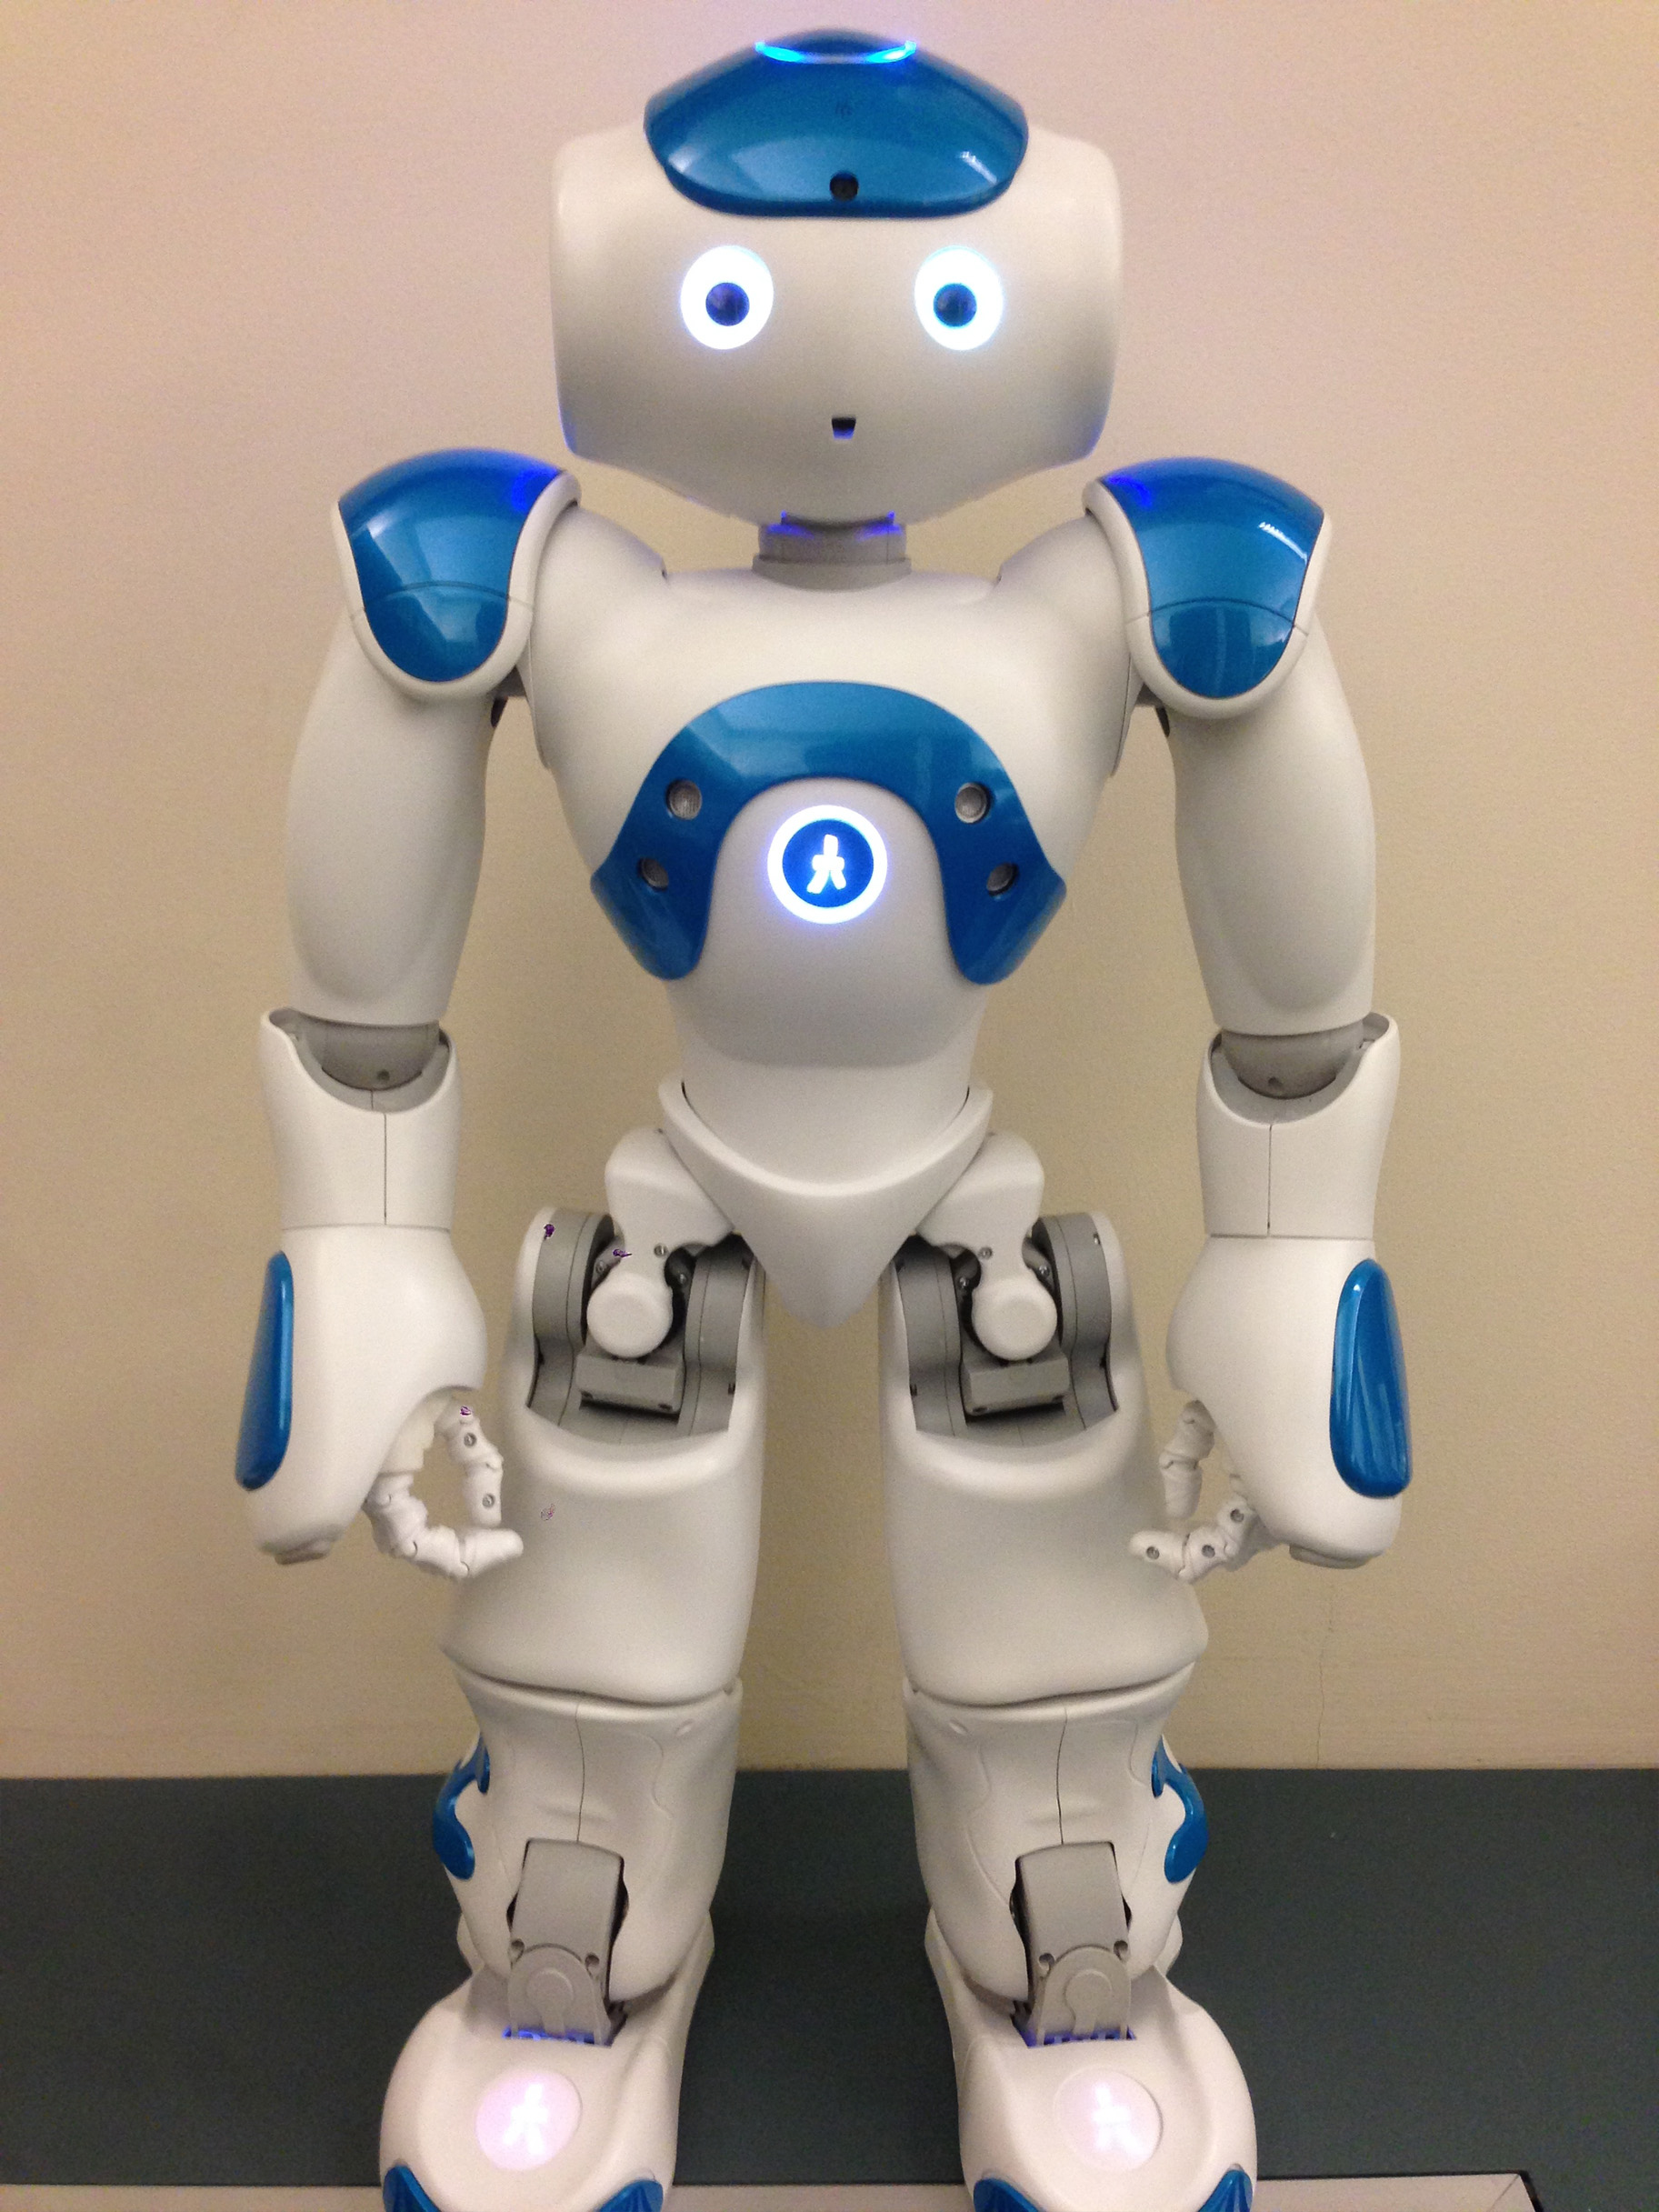
\includegraphics[width = 2.1in]{images/1.jpg}}&
\subfloat[hips]{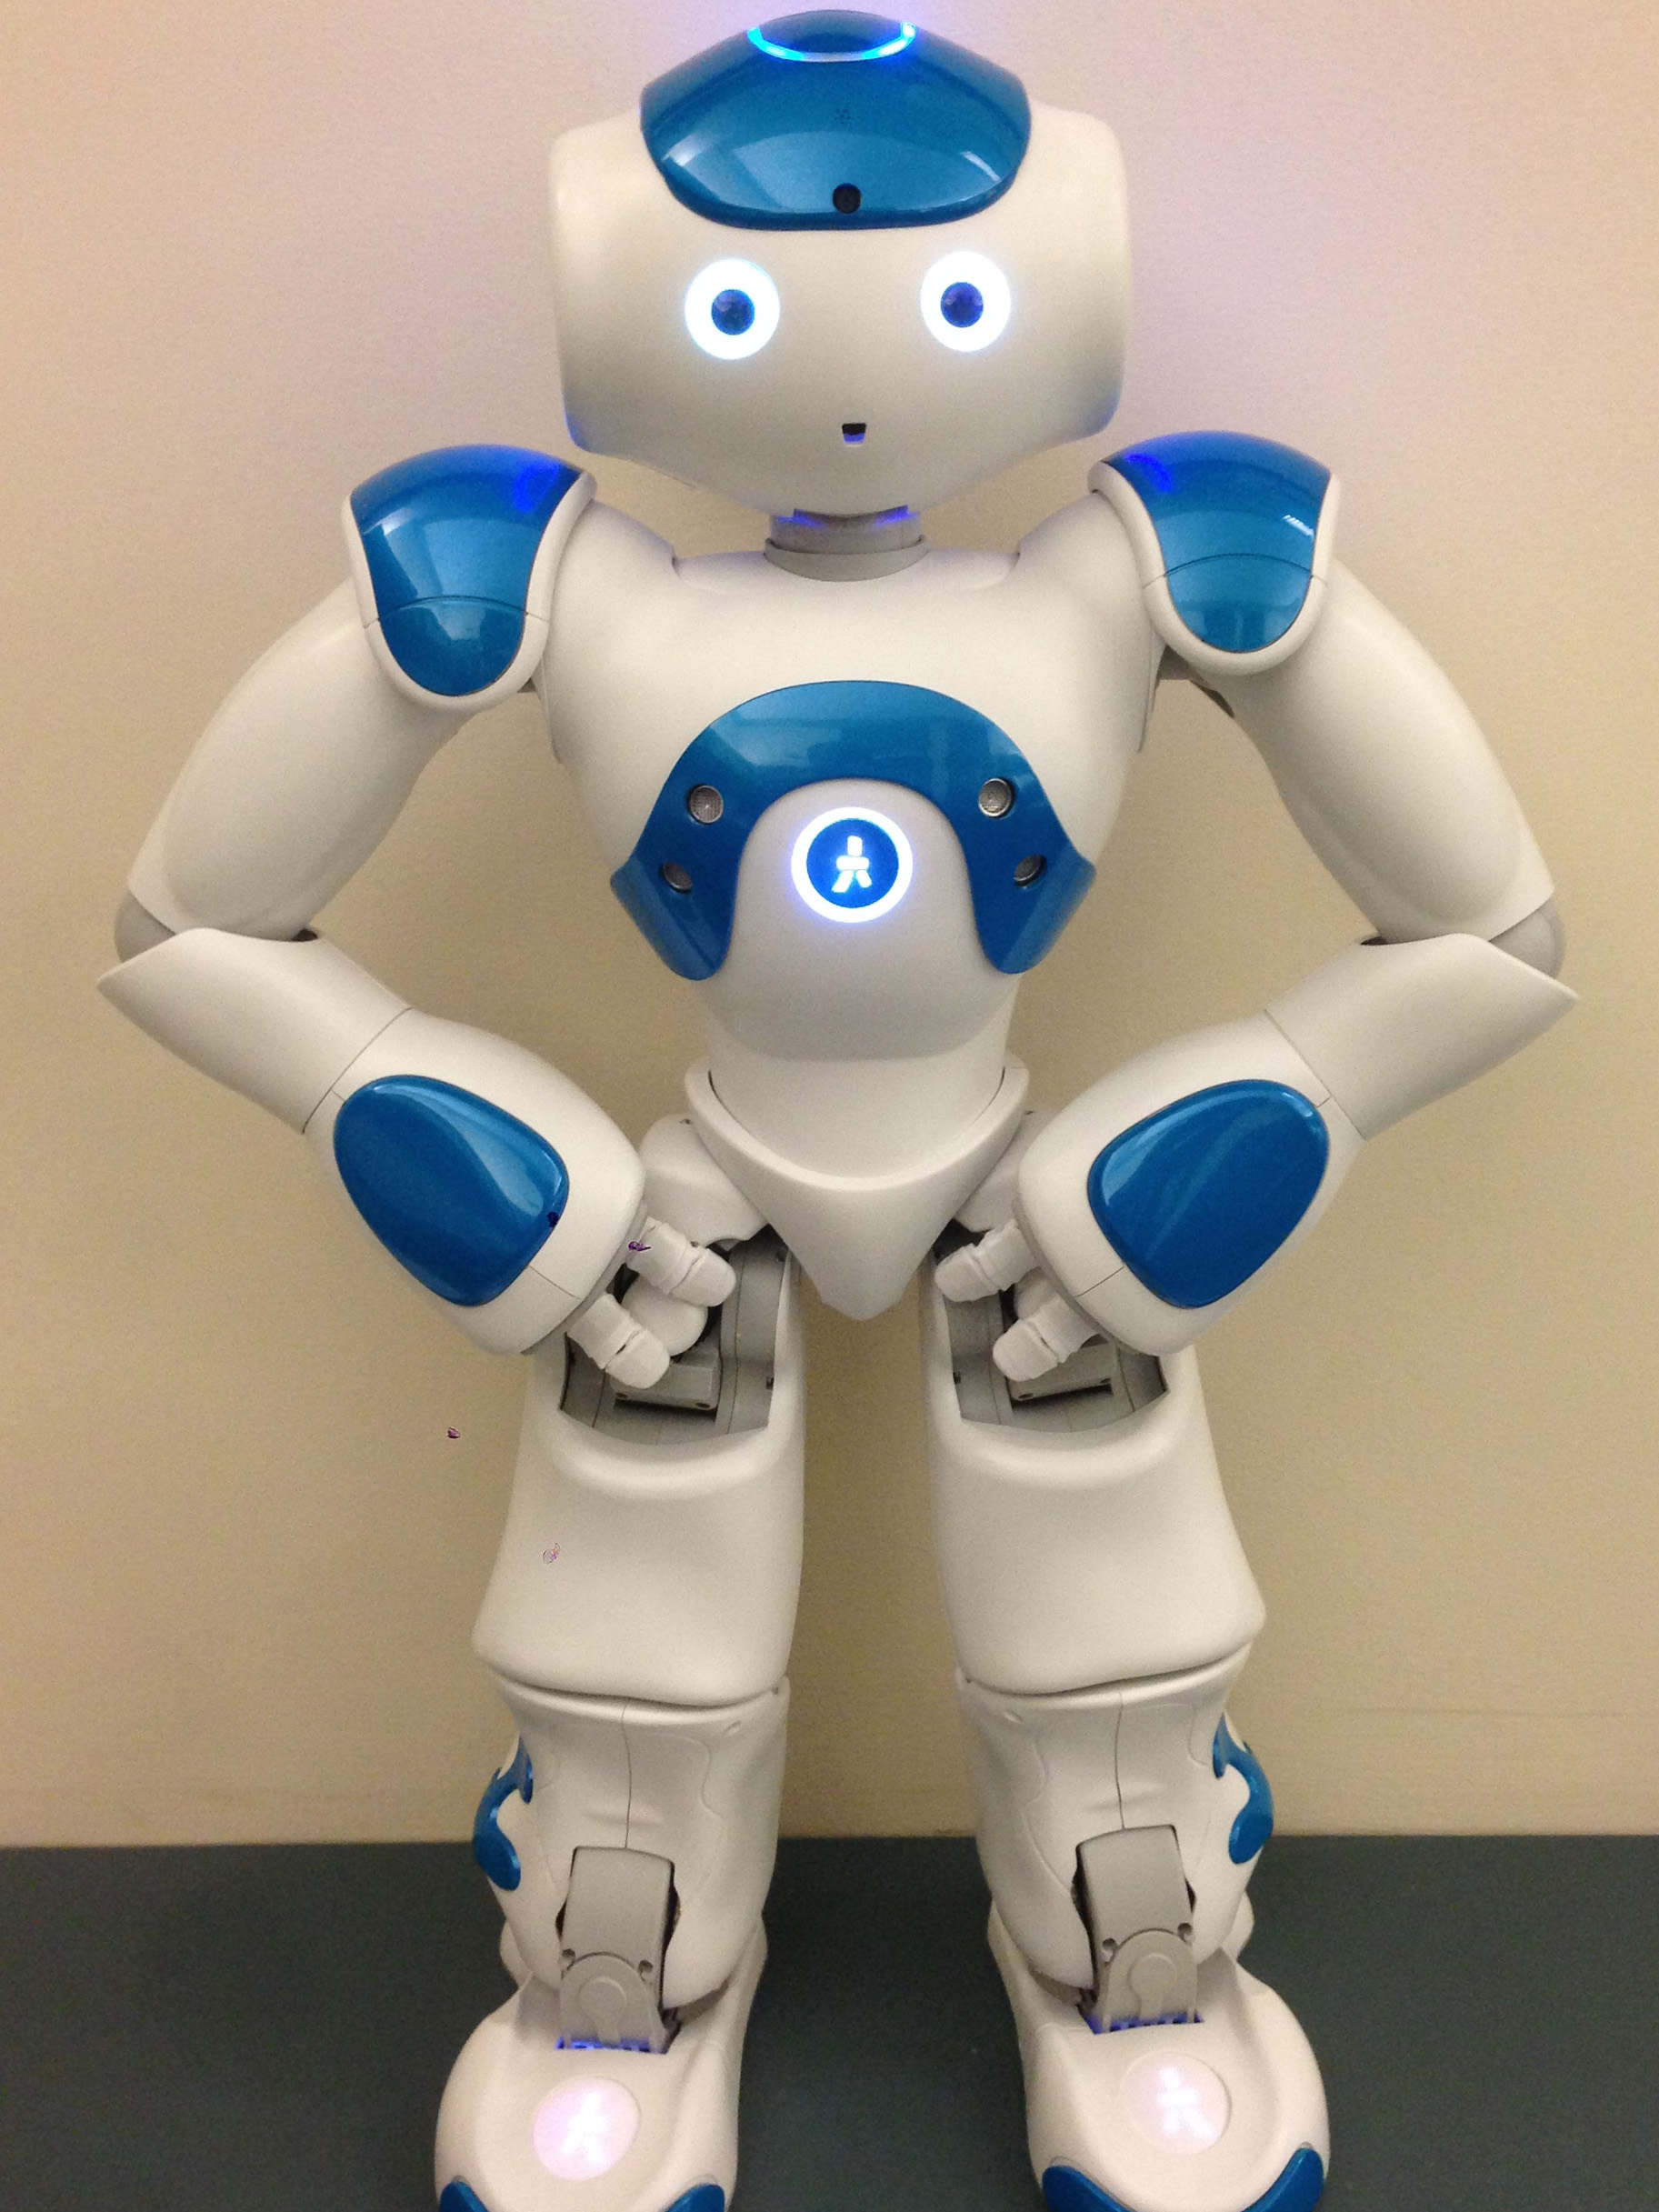
\includegraphics[width = 2.1in]{images/2.jpg}}&
\subfloat[back]{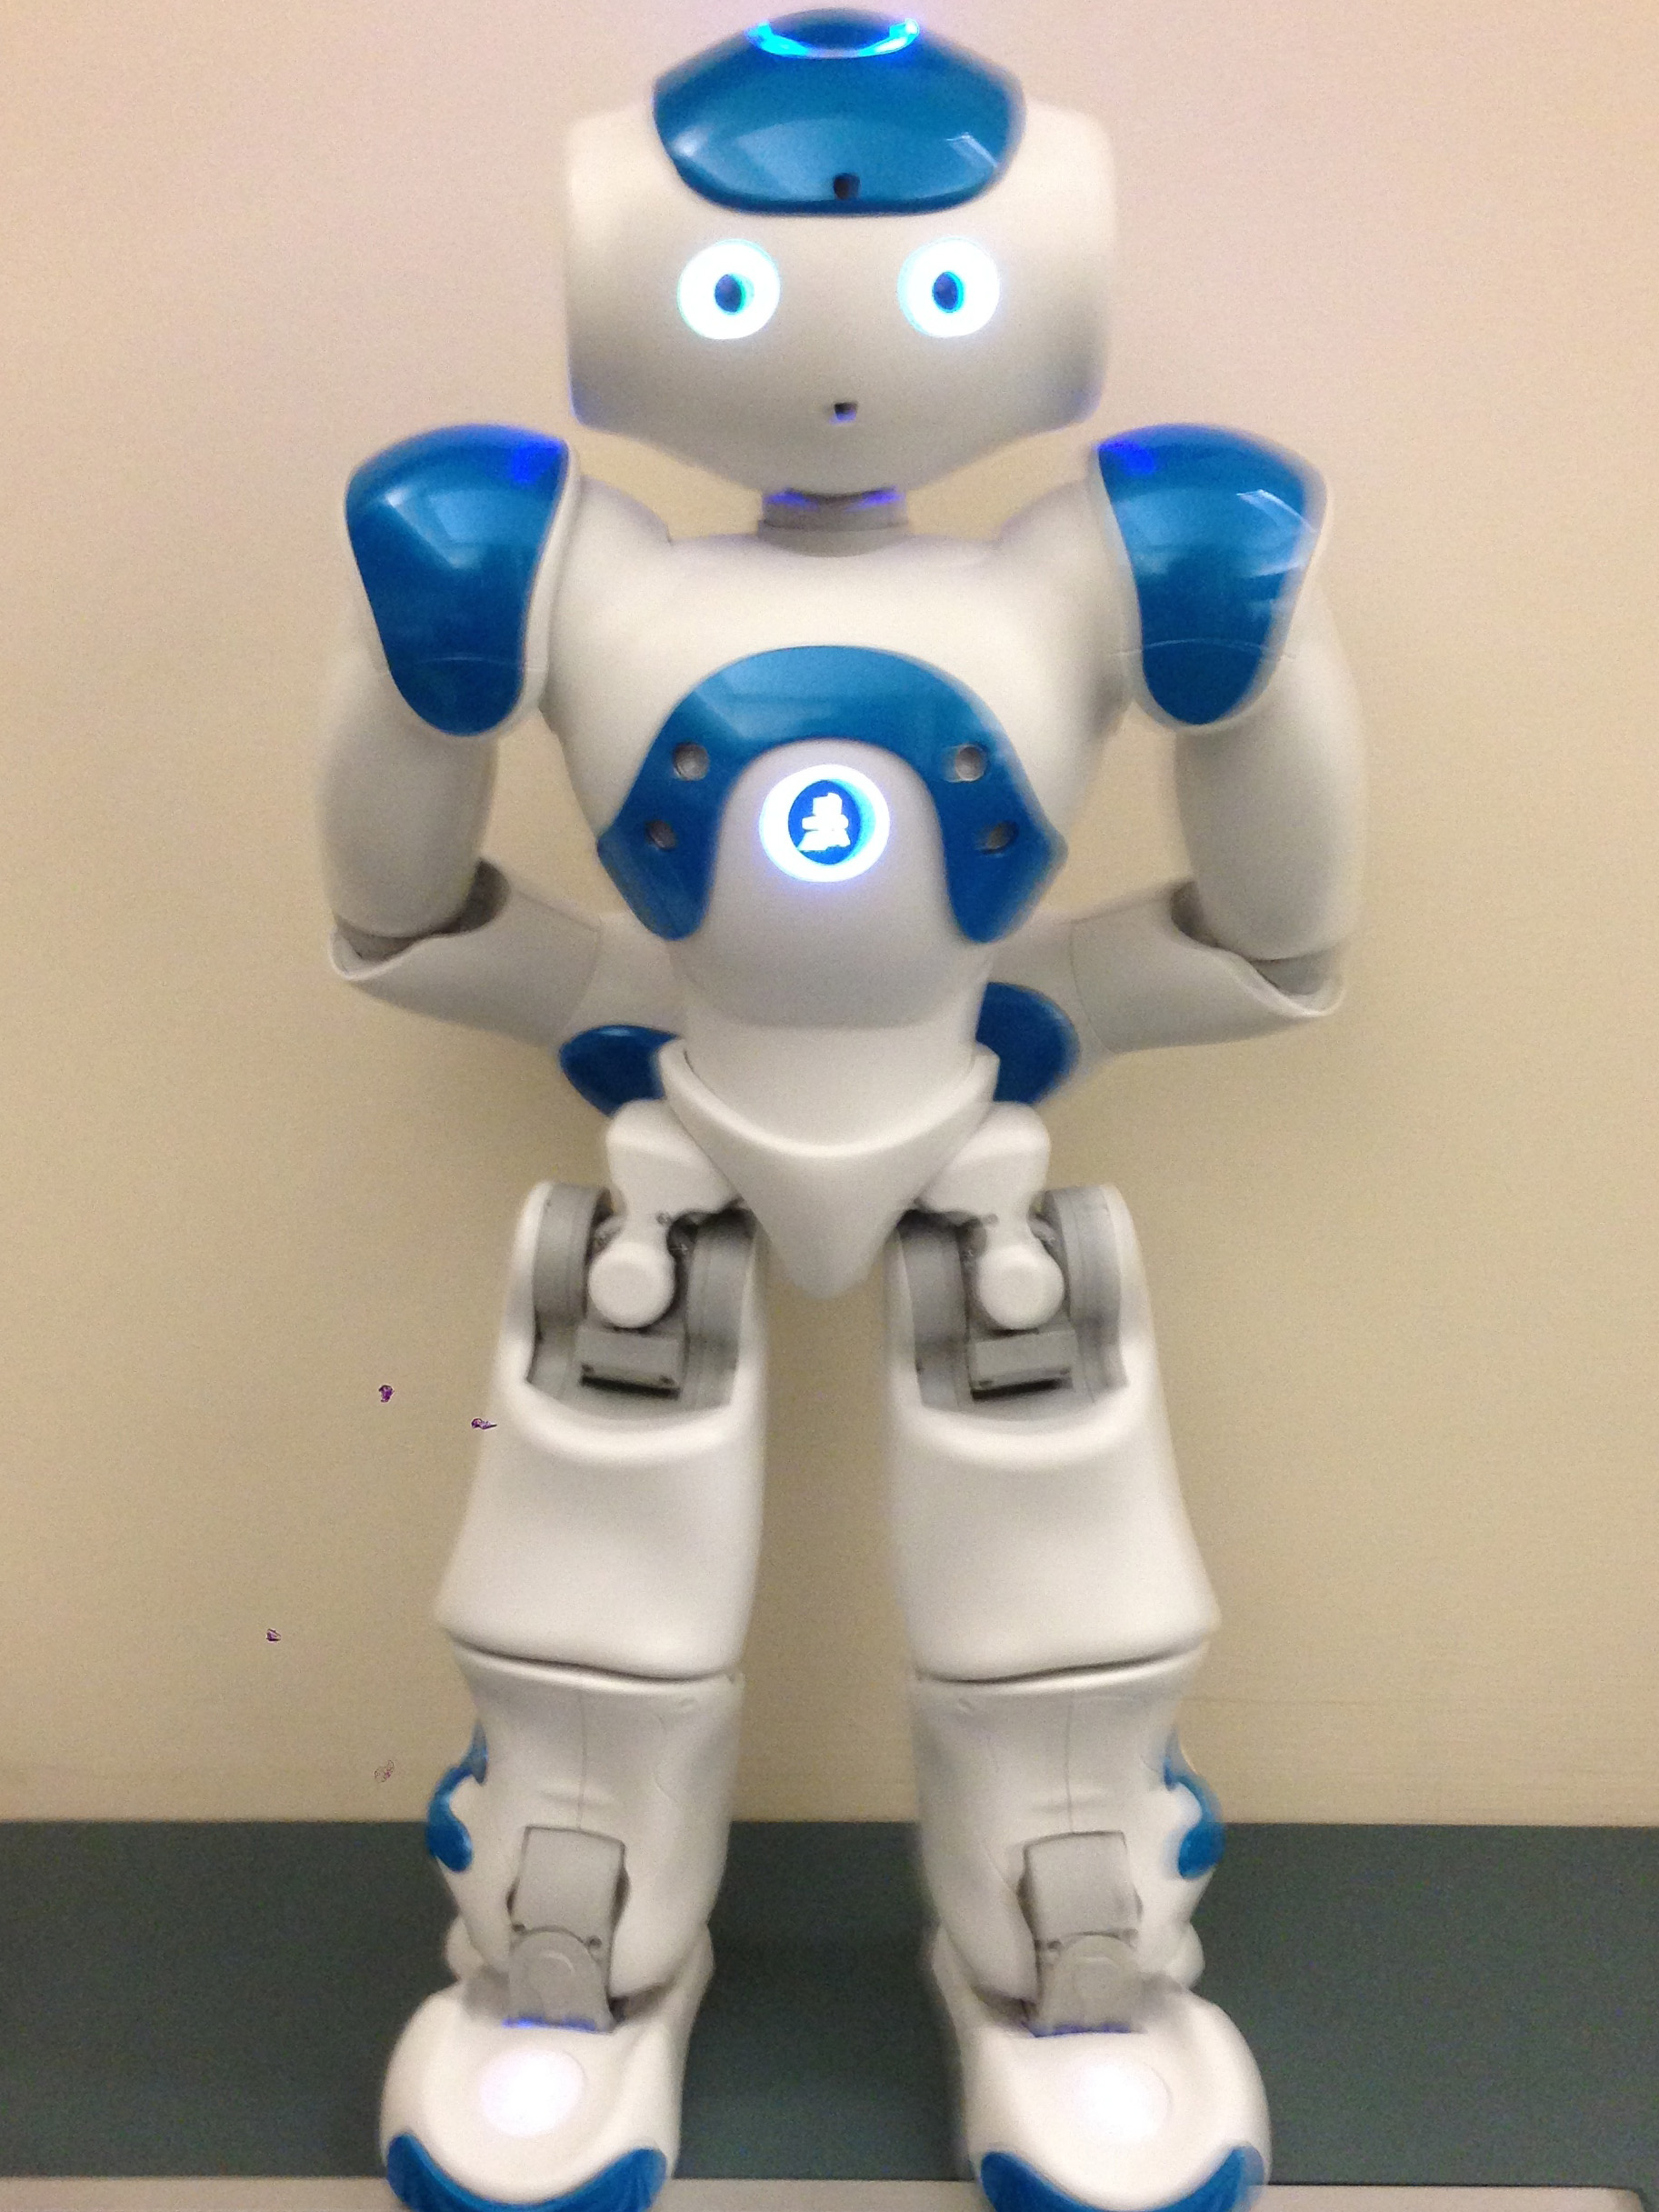
\includegraphics[width = 2.1in]{images/3.jpg}}
\end{tabular}
\caption{Nao Robot Displaying Different Behaviors}
\label{nao}
\end{figure*}

Our study borrows its experimental design from Chartrand \& Bargh \cite{chartrand1999chameleon} but uses a robot in the role of the confederate. The participants were given the task of describing paintings together with the robot. The robot performs one of two behaviors while describing paintings. It either puts its hands on its hips or behind its back. We measure the time the participants put their hands on their hips or behind their backs both before and after the robot does so and we look for the difference between the two.

We initially ran a pilot study from which we observed there were two groups of people, those who spontaneously performed a behavior without the robot doing so and those who did not. In particular, we observed that those who did not spontaneously perform a behavior started doing so after seeing the robot display it and that those who did spontaneously perform a behavior started doing so less after seeing the robot display it. We thus define spontaneous exhibition of a behavior to be performing a specified behavior for any period of time prior to observing the robot perform said behavior.

Based on this, we hypothesized the following:\\
\textbf{H1}	People who do not spontaneously exhibit a behavior will perform that behavior more after seeing a robot perform it.\\
\textbf{H2} People who do spontaneously exhibit a behavior will perform that behavior less after seeing a robot perform it.

For this experiment our robot platform was a Nao, a 58-cm tall humanoid robot, as shown in figure~\ref{nao}(a), designed by Aldebaran on the Naoqi operating system \cite{naodocumentation}. Nao has 25 degrees of freedom, 2 cameras, 4 microphones, speakers, touch sensors, and an inertial measurement unit \cite{naodocumentation}. For the study, Nao's legs were employed for standing up, Nao's arms were used to assume 1 of the 2 aforementioned postures, Nao's touch senors were used to start a script of behaviors, and Nao's speakers were used to voice the painting descriptions. Python was used to program the Nao for the study. 

The behaviors we chose for the Nao were hands behind back, as shown in figure~\ref{nao}(c), and hands on hips, as shown in figure~\ref{nao}(b). We coded a participant putting hands on hips with 4 different designations and a participant putting hands behind back with 3 different designations. The different designations ensured we were able to cover all variations of the behaviors in the event they were displayed. For hands on hips the designations were two hands on hips, one hand on hip, hands in pockets, and hands in belt loops. We ultimately did not use hands in pockets or hands in belt loops because they did not accurately resemble the Nao's behavior. For hands behind back the designations were two hands behind back, one hand behind back, and hands in back pockets. We ultimately did not use hands in back pockets because it did not accurately resemble the Nao's behavior. 

For our analysis we broke both behaviors into a strict and loose definition. For hands on hips, the strict definition matches the Nao's behavior of putting two hands on hips. The loose definition is a superset of this, with the participant exhibiting \textit{at least} one hand on hip. For hands behind back, the strict definition matches the Nao's behavior of putting two hands behind back. The loose definition is a superset of this, with the participant exhibiting \textit{at least} one hand behind back. Having a strict and loose interpretation allowed us to take into account participants who partially performed the behavior in our analysis. 

Participants were first asked to fill out consent and video release forms. Participants were randomly assigned to a group that saw hands behind back or hands on hips during the first session (with the other behavior occurring in the second session). Participants were brought in to a closed 420 cm x 300 cm room. The setup of the room can be seen in figure~\ref{setup}. Participants faced the Nao at a distance of 180 cm. The Nao stood on a platform raised 75 cm off the ground. Next to the Nao stood a 68 cm Apple iMac monitor which ran Python scripts for the Nao's behaviors through a local area network connected to the Nao's head and displayed a PowerPoint presentation on Keynote. The monitor was placed immediately adjacent to the Nao to ensure that participants could describe the paintings without missing the Nao perform its gestures. A GoPro was located at the back of the room and aimed at the participant's back. A camcorder was placed in the corner of the room facing the participant.

The participant was asked to read the first slide of directions while the experimenter turned on the cameras. The directions told the participant that the Nao would describe the painting for 1 minute and that the participant would then describe painting for one minute. The participant was told not to speak while the Nao was speaking. The participant was also told that he or she could repeat what the Nao said. Next, the experimenter started the PowerPoint and tapped the Nao's head sensor to start the Nao's Python scripts. The PowerPoint slides and scripts were synchronized. The Nao would turn its head to ``see'' the painting, turn back to the participant, and describe a painting (descriptions were pre-scripted) for 1 minute after which the participant was notified on-screen to do so as well. The Nao displayed no other idle behaviors while describing paintings or while the participant described paintings. This continued for 3 paintings total. At this point, the Nao performed the assigned behavior and maintained that posture for 3 more paintings while also turning its head to ``see'' the painting at the start of its turn. Thereby, half of the time (3 paintings worth) was before the Nao performed the behavior and half of the team was after the Nao performed the behavior. After 6 total paintings, the Nao returned to a crouch position and the experimenter replaced the Nao with a new one. The same process was repeated with 6 more paintings, except the other behavior was performed in session 2. 

Employing two separate Naos came from the use of two different confederates in the Chartrand \& Bargh study, which also had two different behaviors (touching the face and tapping the feet) \cite{chartrand1999chameleon}. The use of continuous postures (like hands on hips) rather than a discrete behavior (like tapping feet, which can be counted) was largely due to limitations of the robot, but we had little to reason to believe continuous postures would not be effective behaviors given their use in mimicry research \cite{chartrand2013antecedents}. 

The Nao's descriptions of the paintings were kept to be as simple as possible, with little to no emotion or interpretation \cite{hofree2014bridging}. The Nao also made no acknowledgement of the participants or their descriptions and the behaviors of hands behind back and hands on hips were chosen to minimize postural communication. This falls in line with our goals for understanding human mimicry of robots at its most basic level.

After both sessions were completed, the participant completed a survey on Qualtrics, received \$5, and left.

\begin{figure}[t!]
\centering
 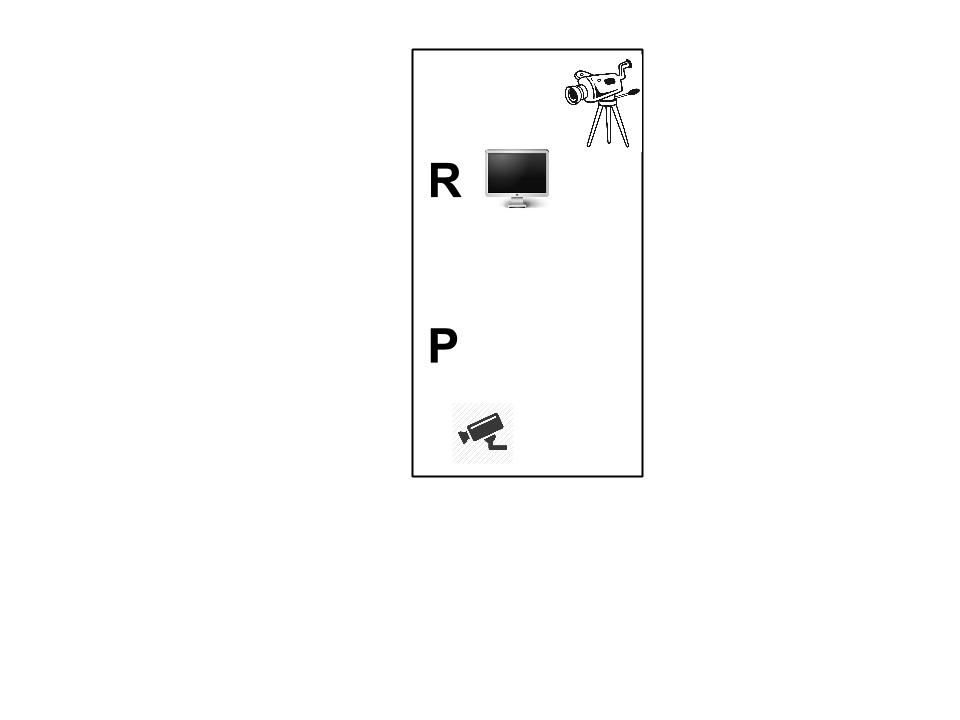
\includegraphics[width=1.05\linewidth]{images/setup.jpg}\\
 \caption{Experimental Setup of the Room}
 \label{setup} %\vspace*{-2mm}
\end{figure}

Video of the participants were collected through a camcorder that captured the front of the participant and a GoPro that captured the back of the participant (this was necessary in order to validate any behaviors the participants portrayed behind their backs).

The videos were coded using ELAN 4.7.3. Both behaviors and variations of the behaviors were coded for. Participants also filled out a survey comprising of Likert Scale questions on intelligence and likability, short answer questions on what they liked/noticed about the trial, and demographic questions. Participants comprised of 47 undergraduates of which 43 were used in the final data analysis (4 participants did not qualify for the study or experienced a technical problem, such as losing internet connection, during the trial).

\section{Results}
The central question of this study is whether or not a robot can induce mimicry in humans. This experiment yielded quantitative results from video coding of the recordings of participants and from self-reporting through a survey of Likert scale and short-answer questions. 

\textbf{Statistical Methods} Our determinations for statistical significance used the following guidelines and justifications. 
%P-values less than 0.05 were deemed statistically significant while p-values between 0.05 and 0.1 were deemed marginally significant. 
Given that the experiment was run as a within-subjects study, a paired t-test was used. We used one-tailed t-tests because of our division of spontaneous and non-spontaneous participants based on their performance of a behavior being 0 or positive before the Nao performed the respective behavior. We did this because of the observations we were able to make as a result of our initial pilot, as mentioned in the Methods Section. Thereby, we knew the direction for the spontaneous group would be negative and the direction for the non-spontaneous group would be positive. This justifies our use of a one-tailed t-test. 

For a given participant, the ``before'' period is defined as the time before the Nao performs the specified behavior and the ``after'' period is defined as the time after the nao performs the specified behavior.

\textbf{Hands on Hips} 

For the \textbf{strict} definition of hands on hips, non-spontaneous participants performed the behavior more in the ``after'' period (\textit{M} = 9280.71 ms, \textit{SD} = 21273.90 ms) than in the ``before'' period (\textit{M} = 0.00 ms, \textit{SD} = 0.00 ms), \textit{t}(33) = 2.54, \textit{p} = 0.008.

For the \textbf{strict} definition of hands on hips, spontaneous participants performed the behavior less in the ``after'' period (\textit{M} = 42047.00 ms, \textit{SD} = 59608.97 ms) than in the ``before'' period (\textit{M} = 90381.00 ms, \textit{SD} = 88705.54 ms), \textit{t}(8) = 2.29, \textit{p} = 0.026.

The results for the strict definition of hands on hips, both non-spontaneous and spontaneous, are shown in figure~\ref{hips}.

For the \textbf{loose} definition of hands on hips, non-spontaneous participants performed the behavior more in the ``after'' period (\textit{M} = 11592.13 ms, \textit{SD} = 25920.62 ms) than in the ``before'' period (\textit{M} = 0.00 ms, \textit{SD} = 0.00 ms), \textit{t}(32) = 2.53, \textit{p} = 0.008.

For the \textbf{loose} definition of hands on hips, spontaneous participants performed the behavior less in the ``after'' period (\textit{M} = 39655.36 ms, \textit{SD} = 64828.17 ms) than in the ``before'' period (\textit{M} = 80540.36 ms, \textit{SD} = 92746.96 ms), \textit{t}(10) = 2.11, \textit{p} = 0.030.

The results for the loose definition of hands on hips, both non-spontaneous and spontaneous, are shown in figure~\ref{hips}.

\begin{figure}[t!]
\centering
 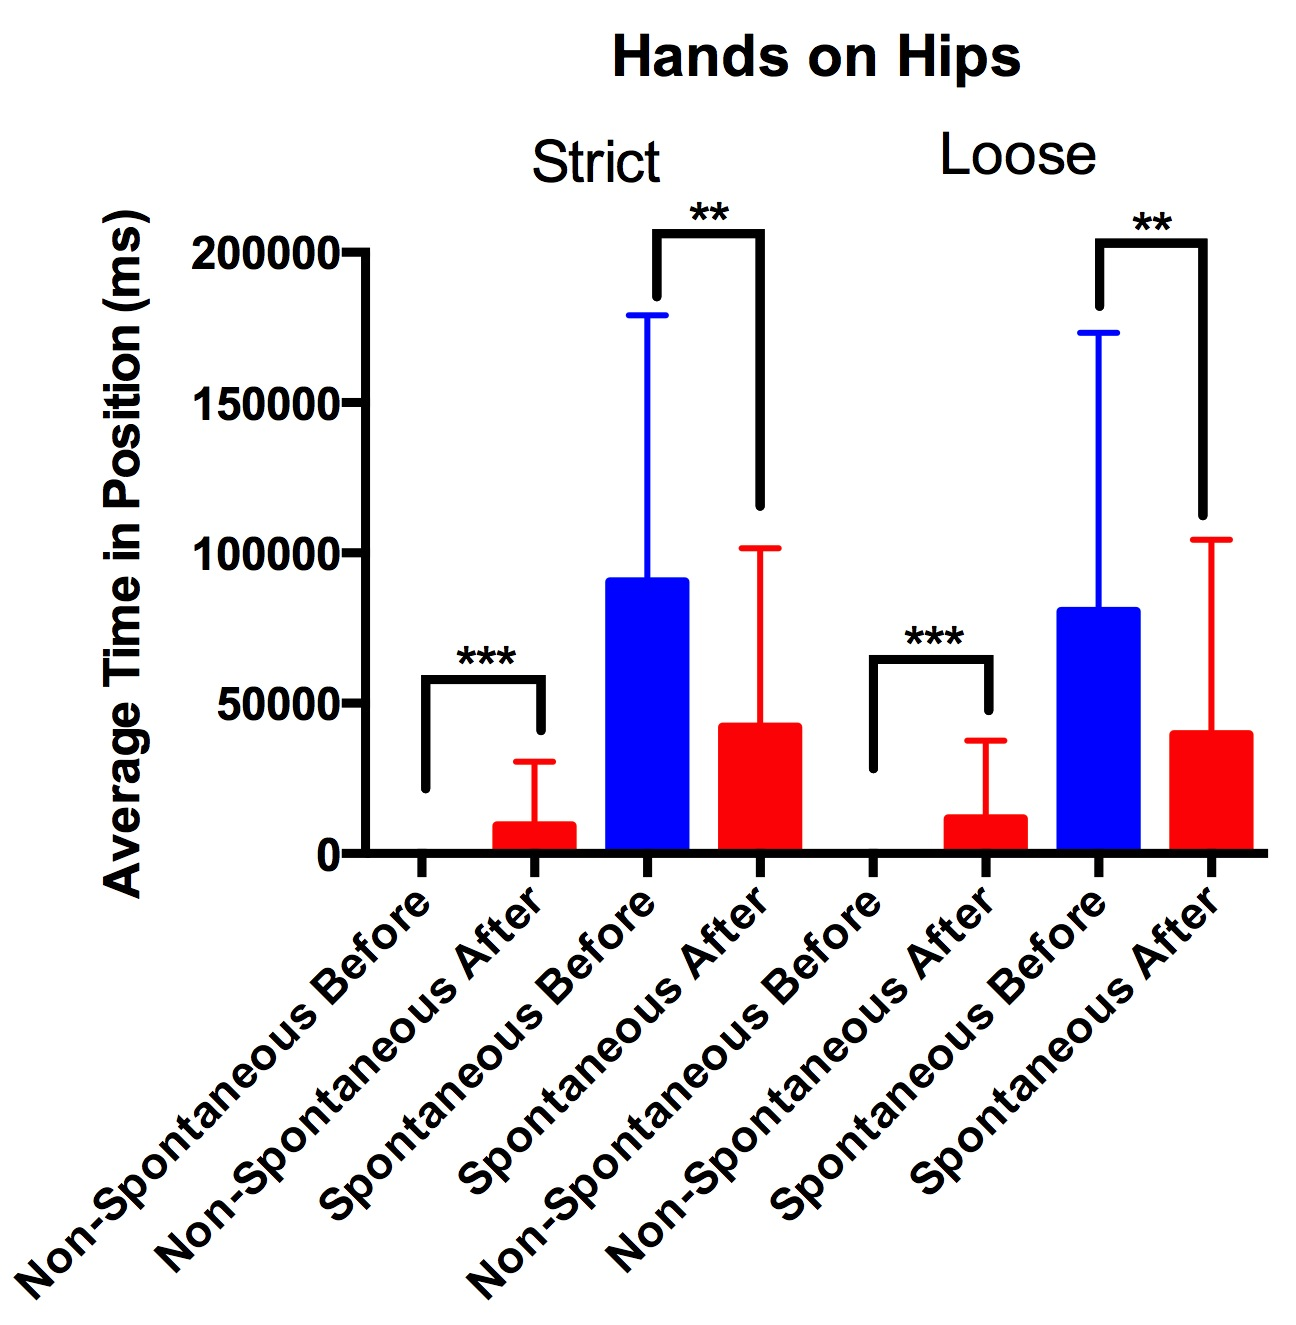
\includegraphics[width=1.00\linewidth]{images/hips.jpg}\\
 \caption{Average time participants perform hands on hips behavior before and after the Nao displayed hands on hips for both strict and loose definitions. ** represents p < 0.05, *** represents p < 0.01} 
 \label{hips} %\vspace*{-2mm}
\end{figure}

\textbf{Hands Behind Back}

For the \textbf{strict} definition of hands behind back, non-spontaneous participants performed the behavior more in the ``after'' period (\textit{M} = 13420.10 ms, \textit{SD} = 47423.54 ms) than in the ``before'' period (\textit{M} = 0.00 ms, \textit{SD} = 0.00 ms), \textit{t}(29) = 1.55, \textit{p} = 0.066.

For the \textbf{strict} definition of hands behind back, spontaneous participants performed the behavior less in the ``after'' period (\textit{M} = 49043.77 ms, \textit{SD} = 99975.38 ms) than in the ``before'' period (\textit{M} = 116665.08 ms, \textit{SD} = 144992.65 ms), \textit{t}(12) = 1.91, \textit{p} = 0.040.

The results for the strict definition of hands behind back, both non-spontaneous and spontaneous, are shown in figure~\ref{back}.

For the \textbf{loose} definition of hands behind back, non-spontaneous participants performed the behavior more in the ``after'' period (\textit{M} = 22292.48 ms, \textit{SD} = 63531.61 ms) than in the ``before'' period (\textit{M} = 0.00 ms, \textit{SD} = 0.00 ms), \textit{t}(28) = 1.89, \textit{p} = 0.035.

For the \textbf{loose} definition of hands behind back, spontaneous participants performed the behavior less in the ``after'' period (\textit{M} = 73551.36 ms, \textit{SD} = 116104.35 ms) than in the ``before'' period (\textit{M} = 135802.93 ms, \textit{SD} = 145636.49 ms), \textit{t}(13) = 1.76, \textit{p} = 0.051.

The results for the loose definition of hands behind back, both non-spontaneous and spontaneous, are shown in figure~\ref{back}.

\begin{figure}[t!]
\centering
 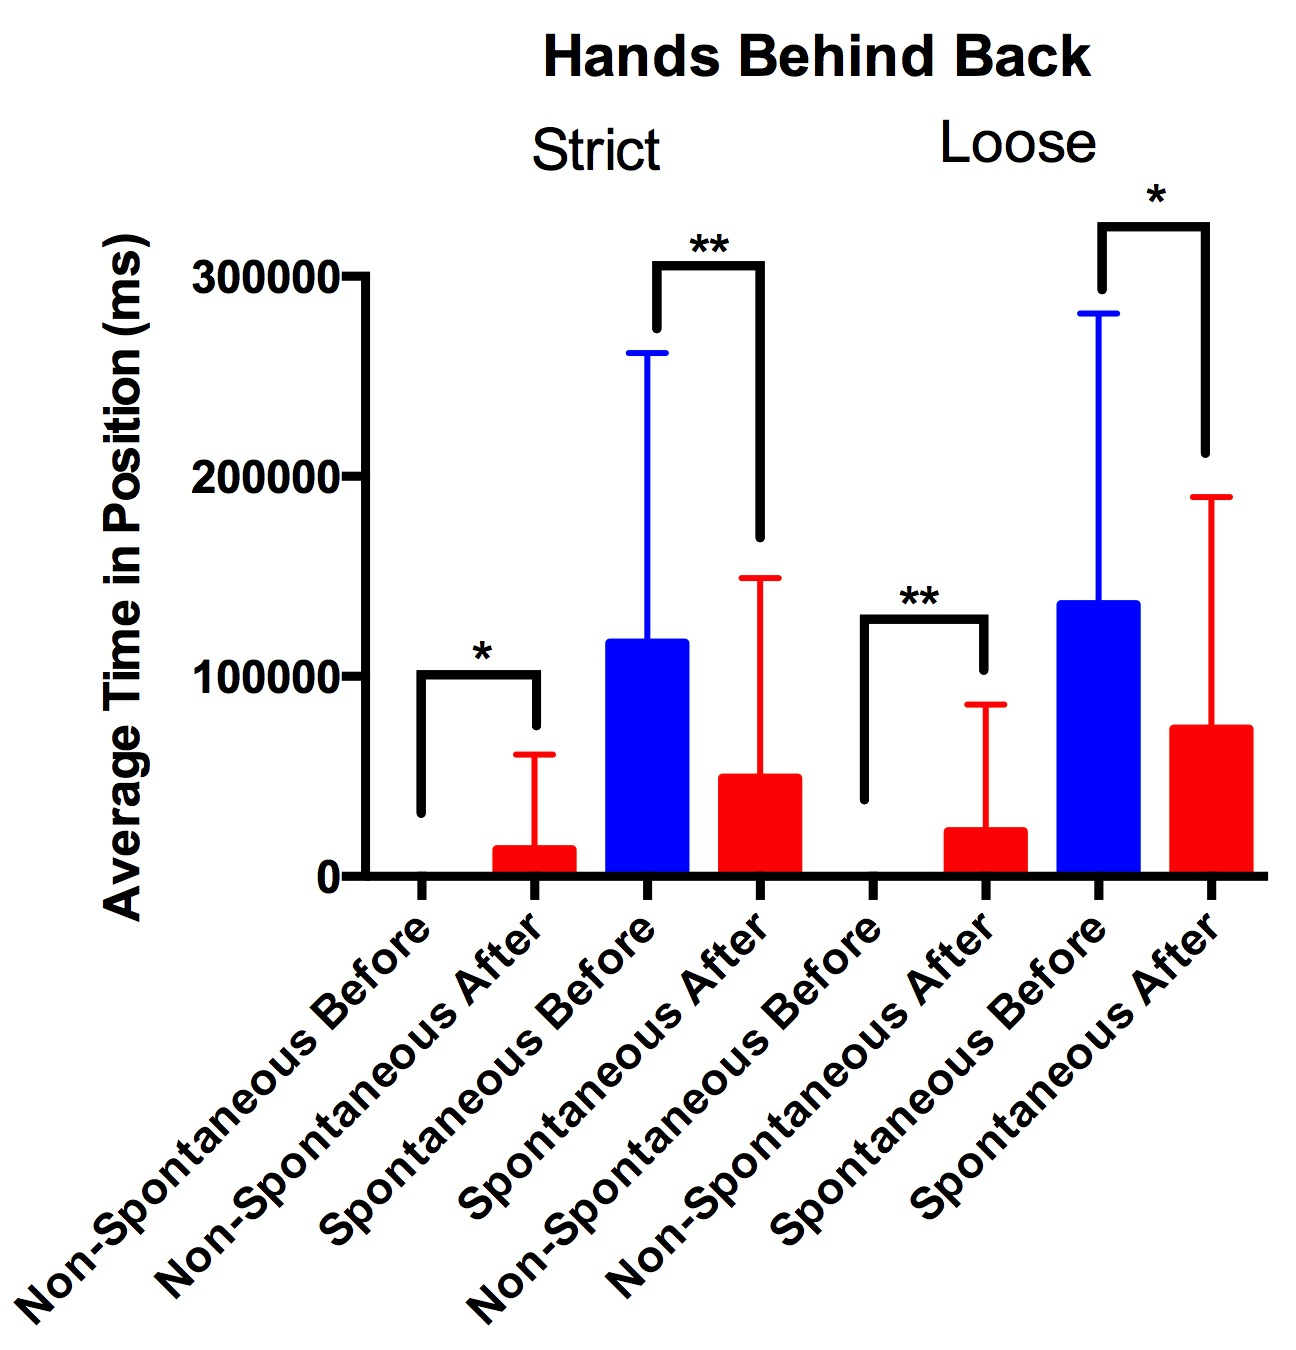
\includegraphics[width=1.00\linewidth]{images/back.jpg}\\
 \caption{Average time participants perform hands behind back behavior before and after the Nao displayed hands behind back for both strict and loose definitions. * represents p < 0.1, ** represents p < 0.05} 
 \label{back} %\vspace*{-2mm}
\end{figure}

\textbf{Survey Results} Beyond providing us insight for our inferences in our discussion, we found no significant result for likability, intelligence, gender, or race and the performance of behaviors before or after the Nao performed them. Our lack of results here can be partially explained by lack of sufficient sample size for questions such as demographic analysis.

\section{Discussion}
Our results yield two main findings about inducing mimicry in humans through robots that support both of our initial hypotheses.
RESULT 1. \textit{Humans who do not spontaneously demonstrate a behavior prior to observing a robot do so perform that behavior more after observing a robot perform it.}
RESULT 2. \textit{Humans who spontaneously demonstrate a behavior prior to observing a robot do so perform that behavior less after observing a robot perform it.}

\textbf{Interpretation of Mimicked Behaviors} Our results support our first hypothesis H1. For both the strict and loose definitions of hands on hips, participants significantly put their hands on their hips more after seeing the Nao do so. This presents very strong evidence for a robot's ability to induce mimicry. For the hands behind back behavior, the strict definition was only marginally significant while the loose definition was statistically significant. This makes sense as the loose definition focuses on the population who put neither hand behind the back, meaning no part of this group even partially performed the behavior spontaneously. Because the loose group focuses on people who in no way perform the behavior spontaneously, their potential for mimicry is maximized in the after period. The differences between strict and loose definitions can be seen in figure~\ref{svl}.

[IS THIS LEGITIMATE]? As far as why the strict definition of hands behind back was only marginally significant while the strict definition of hands on hips was statistically significant, the difference in significance can possibly be explained by the nature of the behaviors themselves. Hands on hips is a more stable behavior in that occurrences of it are longer in duration than the sometimes short burst of hands behind back. This is best captured by the sample size of strict hands on hips vs. strict hands behind back (34 vs. 30). Essentially, there are less participants who by chance or very quickly or casually perform a hands on hips behavior spontaneously. This is especially true with one hand behind back, which is why the loose definition helps to bring hands behind back into statistical significance (the loose definition separates the populations of spontaneous vs. non-spontaneous more thoroughly).

\textbf{Spontaneous Performers Mimic Less} Our results support our second hypothesis H2. This was a surprising yet exciting result of our study. Participants who spontaneously performed hands on hips or hands behind back prior to the Nao doing so actually performed that behavior \textit{less} after the Nao did. While we cannot conclude why this would happen we can make inferences, especially with the help of our survey responses. Several responses noted spontaneous participants saying that when they saw the Nao first put its hands on its hips or put its hands behind its back, they thought the Nao was mimicking their behavior. Such a thought process makes sense when we recall that the spontaneous participants had performed that behavior already at some point before ever seeing the Nao do so. The fact that several participants were trying to figure out the purpose of the study only further pushed them to attribute the Nao's behavior as the Nao mimicking them (albeit in the wrong direction). This stands in contrast to several non-spontaneous participant responses who correctly identified the purpose of the study and did not confuse the direction of mimicry since they had never performed it up until that point. With this idea in hand that participants thought they were being mimicked, we can go back to psychology literature to look for explanations. Mimicry research in psychology has shown that mimicry can lead to socially cold feelings or the feeling that something is ``off''. In particular, an inappropriate amount of mimicry arouses suspicion in the party being mimicked \cite{bargh2012substitutability}, \cite{leander2012you}, \cite{stel2010mimicking}, \cite{zhong2008cold}. This can possibly explain why there is a decrease in performance of hands on hips or hands behind back for spontaneous participants. Another possible explanation is that humans view the Nao as a member of a social outgroup. It is possible that viewing the Nao as a member of an outgroup makes participants who think the Nao is mimicking them feel that the mimicry is inappropriate \cite{kavanagh2011s}.%; however, given that the non-spontaneous group does show some mimicry it is unclear what conclusions can be drawn about social ingroup/outgroup status of the Nao and robots more generally.

There are several caveats to consider with the theory that participants had a negative reaction to being mimicked. Previous studies showed positive human reactions to being mimicked by a digital avatar when head posture was mimicked \cite{bailenson2005digital}, which seems contradictory to our possible explanation. In that study, however, the mimicking was done on a delay and participants were not aware of the mimicry \cite{bailenson2005digital}. In our study, participants saw what they thought was an explicit attempt at mimicry. The explicit attempt fits more appropriately with the psychology research that discusses problems with ``inappropriate'' amounts of mimicry.

Within the surprising finding for spontaneous performers of the behavior is that the loose definition saw smaller decreases than the strict definition. For hands behind back, the loose definition had such a smaller decrease that it even moved the loose definition for spontaneous participants from statistically significant to marginally significant. This can possibly be explained by the fact that our cutoff for spontaneous vs. non-spontaneous was 0. This means that participants who barely performed the behaviors before the Nao did, even for only 1000 milliseconds, were counted in the spontaneous group. These participants had such a low ``before'' time that they could easily have a higher ``after'' time. This could happen just by chance (particularly for hands behind back which had more small bursts of the behavior) or because the participants who performed the behavior for small periods in the ``before'' period did not take the Nao performing the behavior as an attempt at mimicry, silencing the concern of inappropriate mimicry. Fundamentally, this problem is more pronounced given the small sample size for the spontaneous group.

\section{Conclusion}
Understanding mimicry in human-robot interaction is an essential piece of designing social robots. In particular, mimicry needs to be actively considered in design paradigms and when analyzing the social impact of a robot. In light of this, we ran a study to observe the ability of a robot to induce mimicry in humans. Participants described paintings while interacting with a robot that assumed the posture of either hands on hips or hands behind back. Based on an initial pilot, we identified two groups of people within our sample: those who spontaneously exhibited hands on hips or hands behind back and those who did not. Our study produced two findings. People who did not spontaneously exhibit a behavior, mimicked the robot doing the behavior. People who spontaneously exhibited a behavior, performed the behavior less after observing the robot did the behavior. We discussed possible explanations for our results and their caveats in the previous section.

\textbf{Implications}
In light of our first finding we can conclude that robots can induce mimicry in humans. This opens a lot of new research possibilities and questions. Does the salience of mimicry in human-robot interaction move in the same patterns as it does in humans? For example, does having a goal to affiliate or similarity between partners induce greater mimicry in human-robot interaction as it does in humans \cite{chartrand2013antecedents}? Our second finding also raises concerns about building mimicry into human-robot interaction, especially in terms of having robots mimic humans. Perhaps there are certain prerequisites that must be fulfilled in a human-robot partnership before mimicry is considered appropriate. Lastly, this study raises issues for design of robots and their impact on humans around them. Just as we are wary of how other humans may mimic our actions, we must be wary of how robots may induce humans to mimic tasks, particularly if they are tasks we design robots to do specifically because we don't want humans doing them.

%ACKNOWLEDGMENTS are optional
%\section{Acknowledgments}
%The authors would like to thank Rachel Protacio and Jessica Yang for their help in the piloting of this study. They would also like to thank John Bargh of Yale University for his foundational work in the Chameleon Effect and for personally helping with the background research for human-human mimicry.

%
% The following two commands are all you need in the
% initial runs of your .tex file to
% produce the bibliography for the citations in your paper.
\bibliographystyle{abbrv}
\bibliography{sigproc}  % sigproc.bib is the name of the Bibliography in this case
% You must have a proper ".bib" file
%  and remember to run:
% latex bibtex latex latex
% to resolve all references
%
% ACM needs 'a single self-contained file'!
\end{document}
%\begin{figure}[t!]
%\centering
% 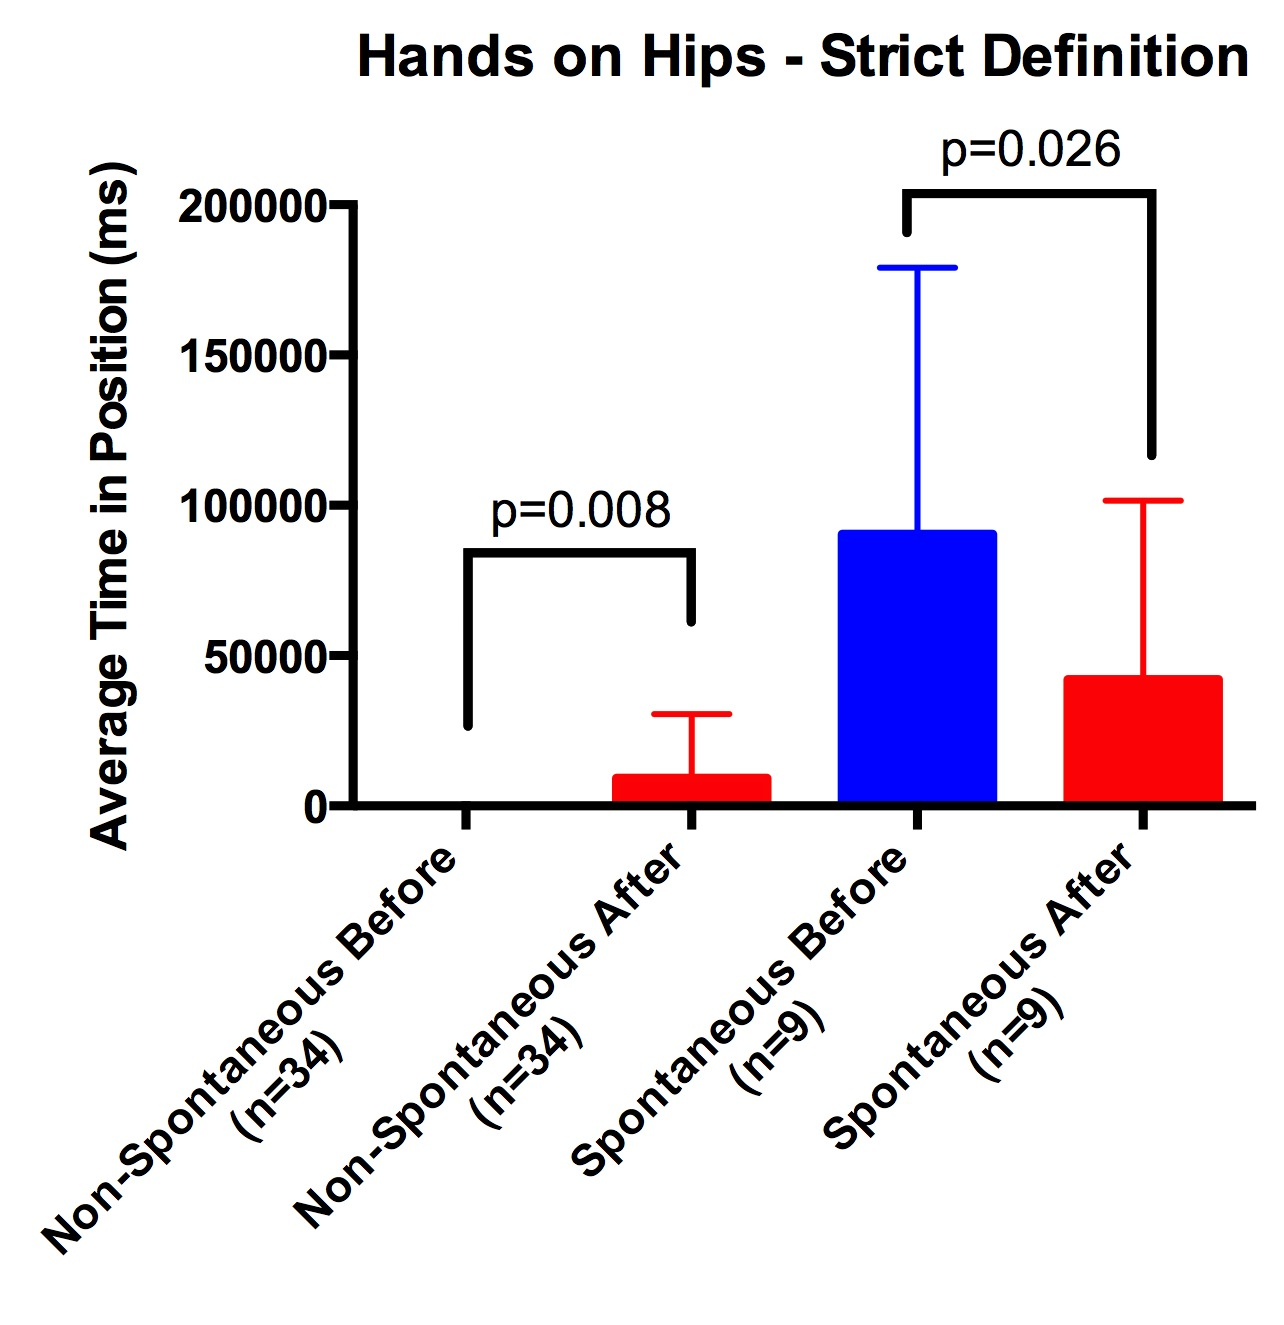
\includegraphics[width=1.00\linewidth]{images/hstrict.jpg}\\
% \caption{Hands on Hips- Strict Definition} 
% \label{hstrict} %\vspace*{-2mm}
%\end{figure}
%\begin{figure}[t!]
%\centering
% 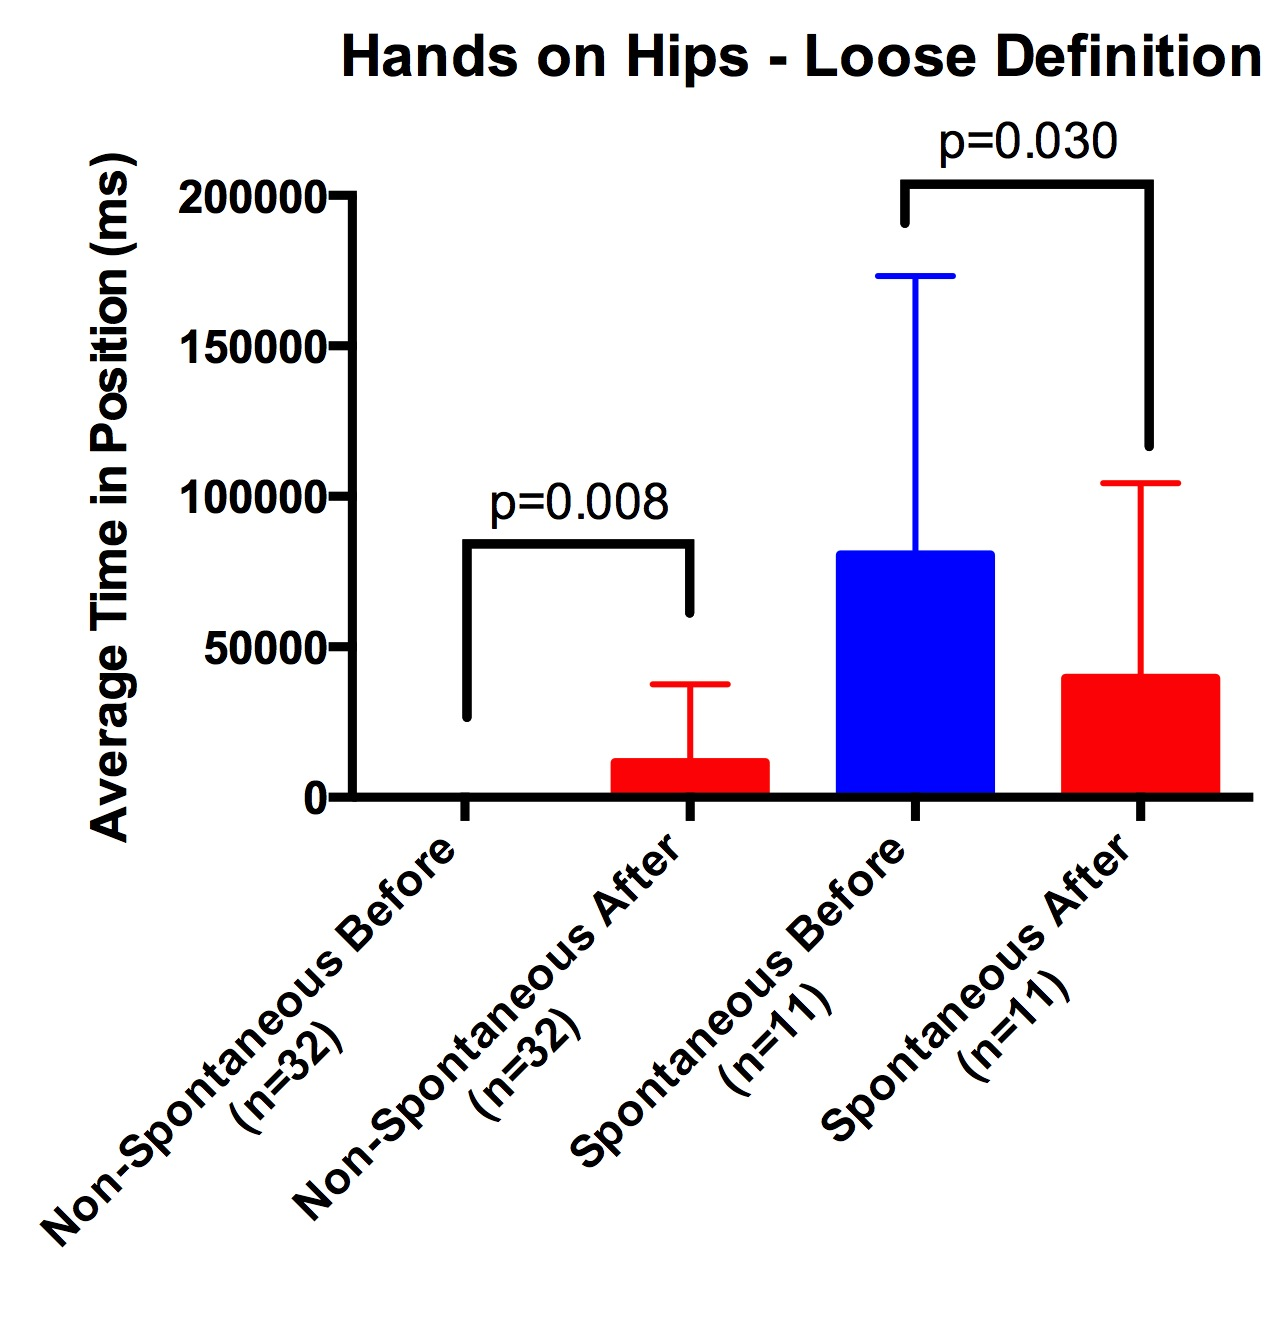
\includegraphics[width=1.00\linewidth]{images/hloose.jpg}\\
% \caption{Hands on Hips - Loose Definition}
% \label{hloose} %\vspace*{-2mm}
%\end{figure}

%\begin{figure}[t!]
%\centering
% 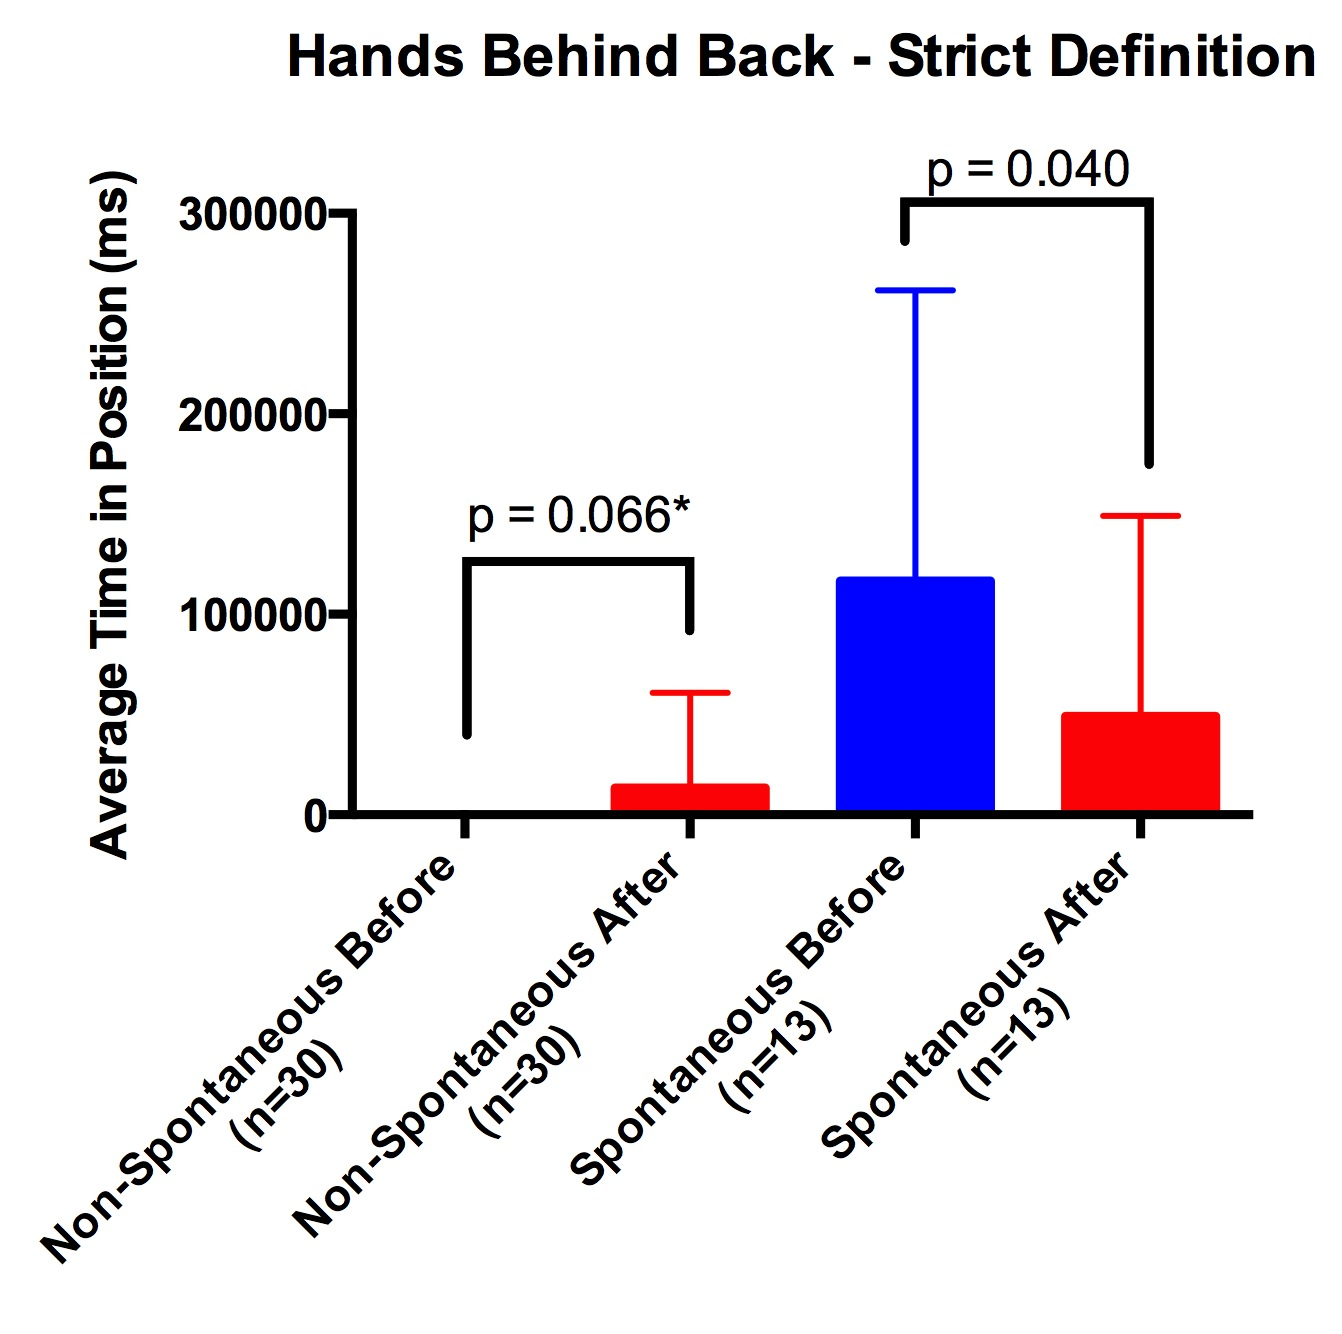
\includegraphics[width=1.00\linewidth]{images/bstrict.jpg}\\
% \caption{Hands Behind Back - Strict Definition}
% \label{bstrict} %\vspace*{-2mm}
%\end{figure}

%\begin{figure}[t!]
%\centering
% 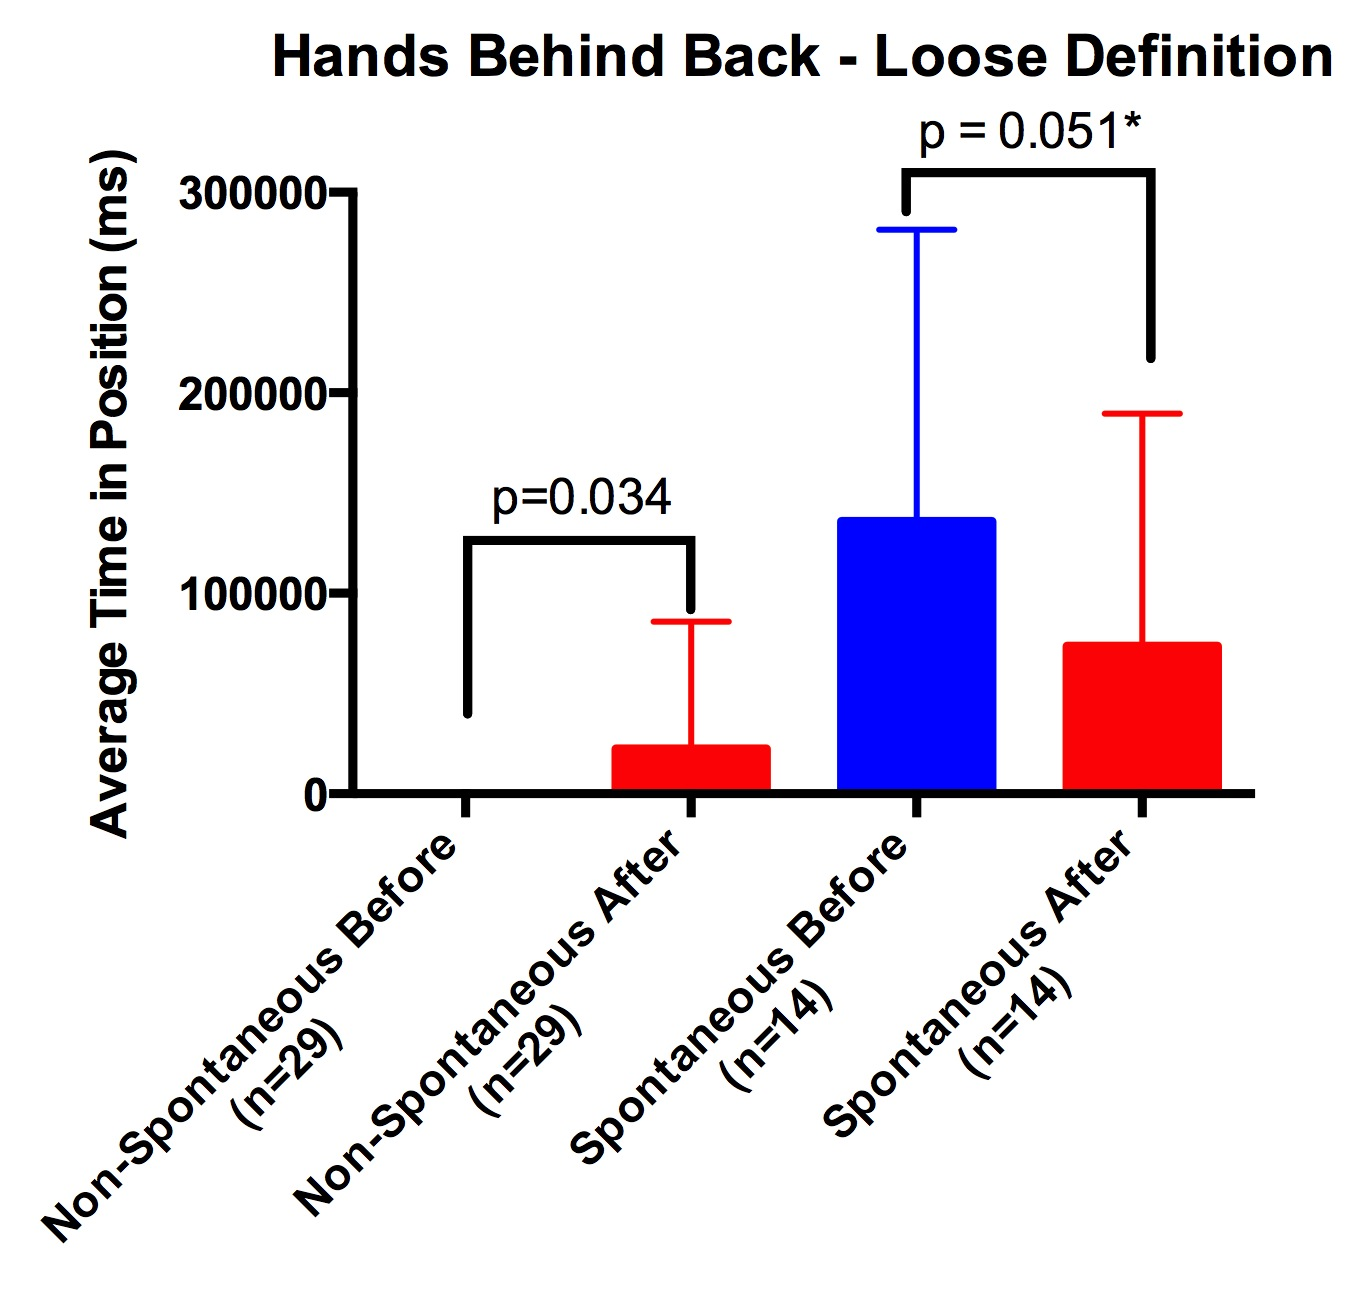
\includegraphics[width=1.00\linewidth]{images/bloose.jpg}\\
% \caption{Hands Behind Back - Loose Definition}
% \label{bloose} %\vspace*{-2mm}
%\end{figure}
%\begin{figure}[t!]
%\centering
% 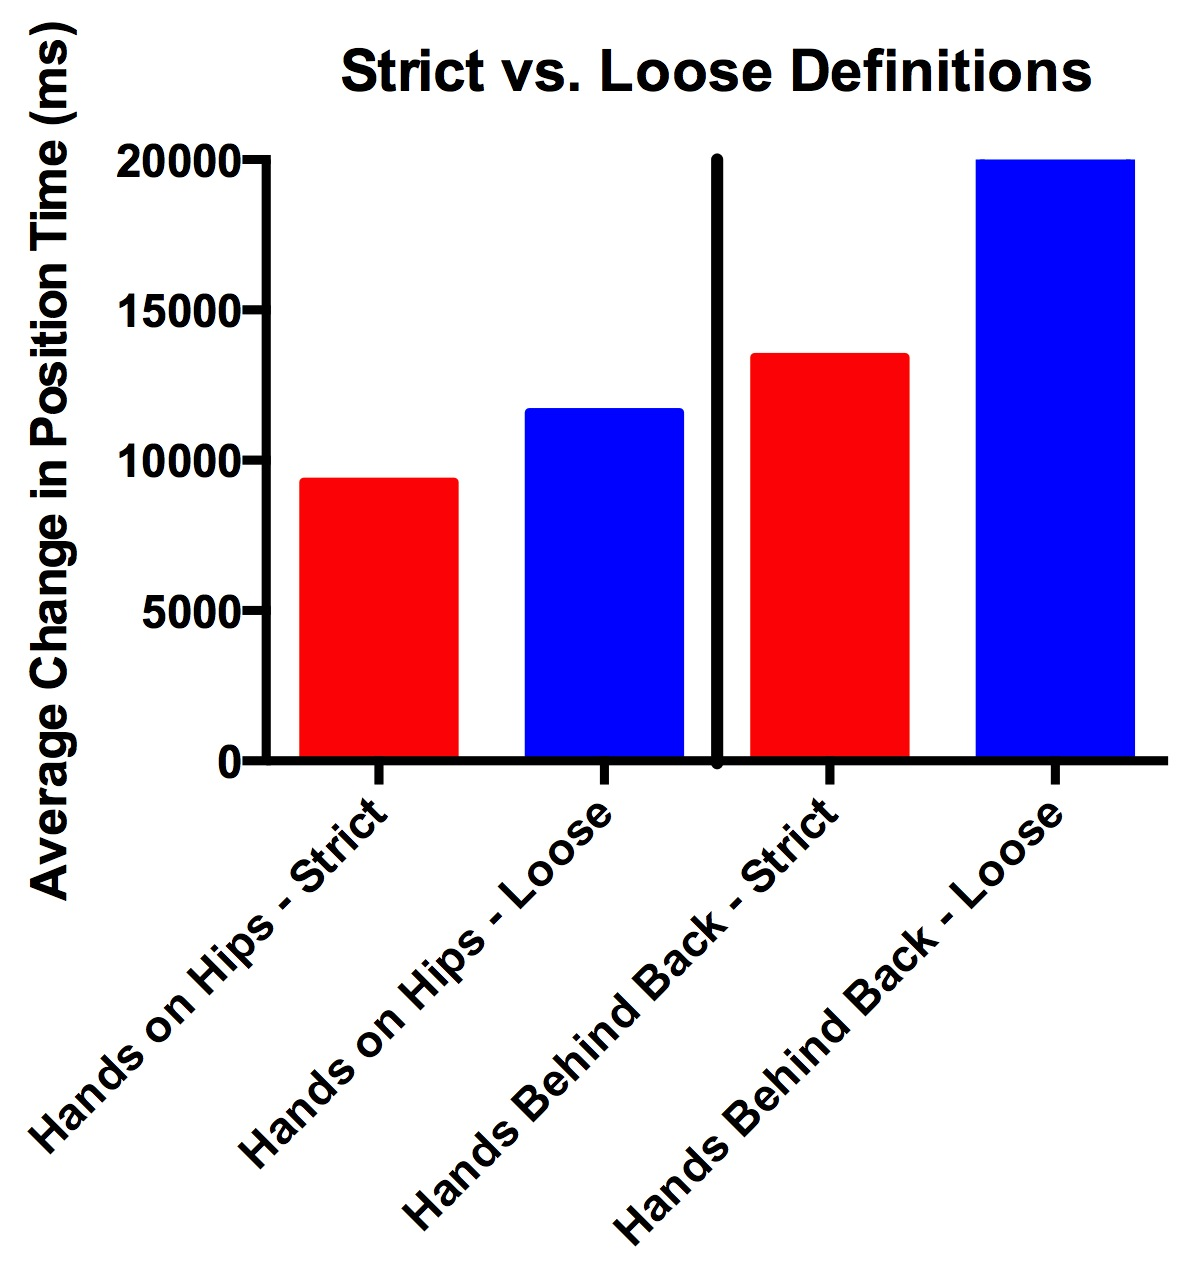
\includegraphics[width=0.85\linewidth]{images/svl.jpg}\\
% \caption{Strict vs. Loose Definitions}
% \label{svl} %\vspace*{-2mm}
%\end{figure}


%In the broadest sense, mimicry is a thinly explored area of human-robot interaction that has a parallel in human-human interaction. Given that psychological research on mimicry has highlighted questions about mimicking the ``right'' people (i.e. ingroups vs. outgroups) \cite{bourgeois2008impact}, \cite{chartrand2013antecedents}, \cite{kavanagh2011s}, \cite{yabar2006implicit}, mimicry could highlight how humans view robots as social actors. 

%!!Also, it has been observed that mimickers, and not just mimickees, \cite{maddux2008chameleons}, \cite{stel2010mimicry}, \cite{swaab2011early} SECTION 3

%From a practical standpoint, if robots can induce mimicry in humans, it provides us insight into how a robot may induce behavior in humans within the real world. One can foresee possible concerns of a child or infant mimicking a robot in the home. One could also foresee issues regarding individuals mimicking a robot in public, perceiving the robot's actions as a sign of permissibility. All these new questions, however, rest on the assumption that a robot could in fact elicit mimicry in humans, an assumption we show to be true in this study. Observing no mimicry or some kind of adverse social effect would also raise questions about why the perception-behavior link in human-human interaction does not extend to human-robot interaction.

%Lastly, mimicry of physical behaviors is the first step in the larger phenomena of social contagion \cite{chartrand2013antecedents}, so understanding how human-robot interaction works for mimicry can act as a stepping stone to social contagion with human-robot interaction.

%Bailenson successfully demonstrated that liking, rapport, and affiliation can be increased with mimicry even with a digital agent, which they showed using a virtual agent on a computer screen mimicking the head posture of the participants \cite{bailenson2005digital}. This highlights one direction of the mimicry effect, in which a participant being mimicked has a more positive experience with a mimicker. The existence of this direction with a non-human agent suggests the possibility of the opposite direction, a human mimicking a non-human agent. 

%Riek conducted a study hoping to observe improved likability with an embodied robot (resembling an ape) mimicking head posture of a participant. Their study identified problems with assessing human-robot interactions using a survey and the difficulties of capturing and mimicking behaviors between humans and robots. Their work guided us in our planning of behaviors \cite{riek2010my}. Riek did find some support for more satisfactory interactions when facial expressions were mimicked by the same ape-like robot, although the findings were preliminary and in a pilot \cite{riek2008real}.

%Participants were given a task to complete while interacting with the robot. Our study borrowed heavily from Chartrand \& Bargh's experimental design \cite{chartrand1999chameleon}. We initially ran a pilot study from which we observed there were two groups of people, those who spontaneously performed a behavior without the robot doing so and those who did not. Knowing this we designed our study as follows.

%We define spontaneous exhibition of a behavior to be performing a specified behavior for any period of time prior to observing the robot perform said behavior. 

%Participants alternated describing paintings with a Nao robot. Halfway through the trial, the Nao would assume a posture (either putting its hands behind its back or putting its hands on its hips) while continuing with the description of paintings. We measured the times the participant assumed the posture before and after the Nao assumed the posture respectively. The ``before'' period acted as the control while the ``after'' period acted as the observed variable, making this a within-subjects study.

%This whole process was repeated with a different Nao for the same participant. The different Nao was brought in by the experimenter immediately after the conclusion of the first session. During the second session, the Nao performed whichever behavior the first Nao did not (either putting its hands behind its back or putting its hands on its hips). This gave us a larger data set of behaviors to observe and also helped us to control for participants who had existing tendencies to do one behavior or another.

%\begin{figure}[t!]
%\centering
% 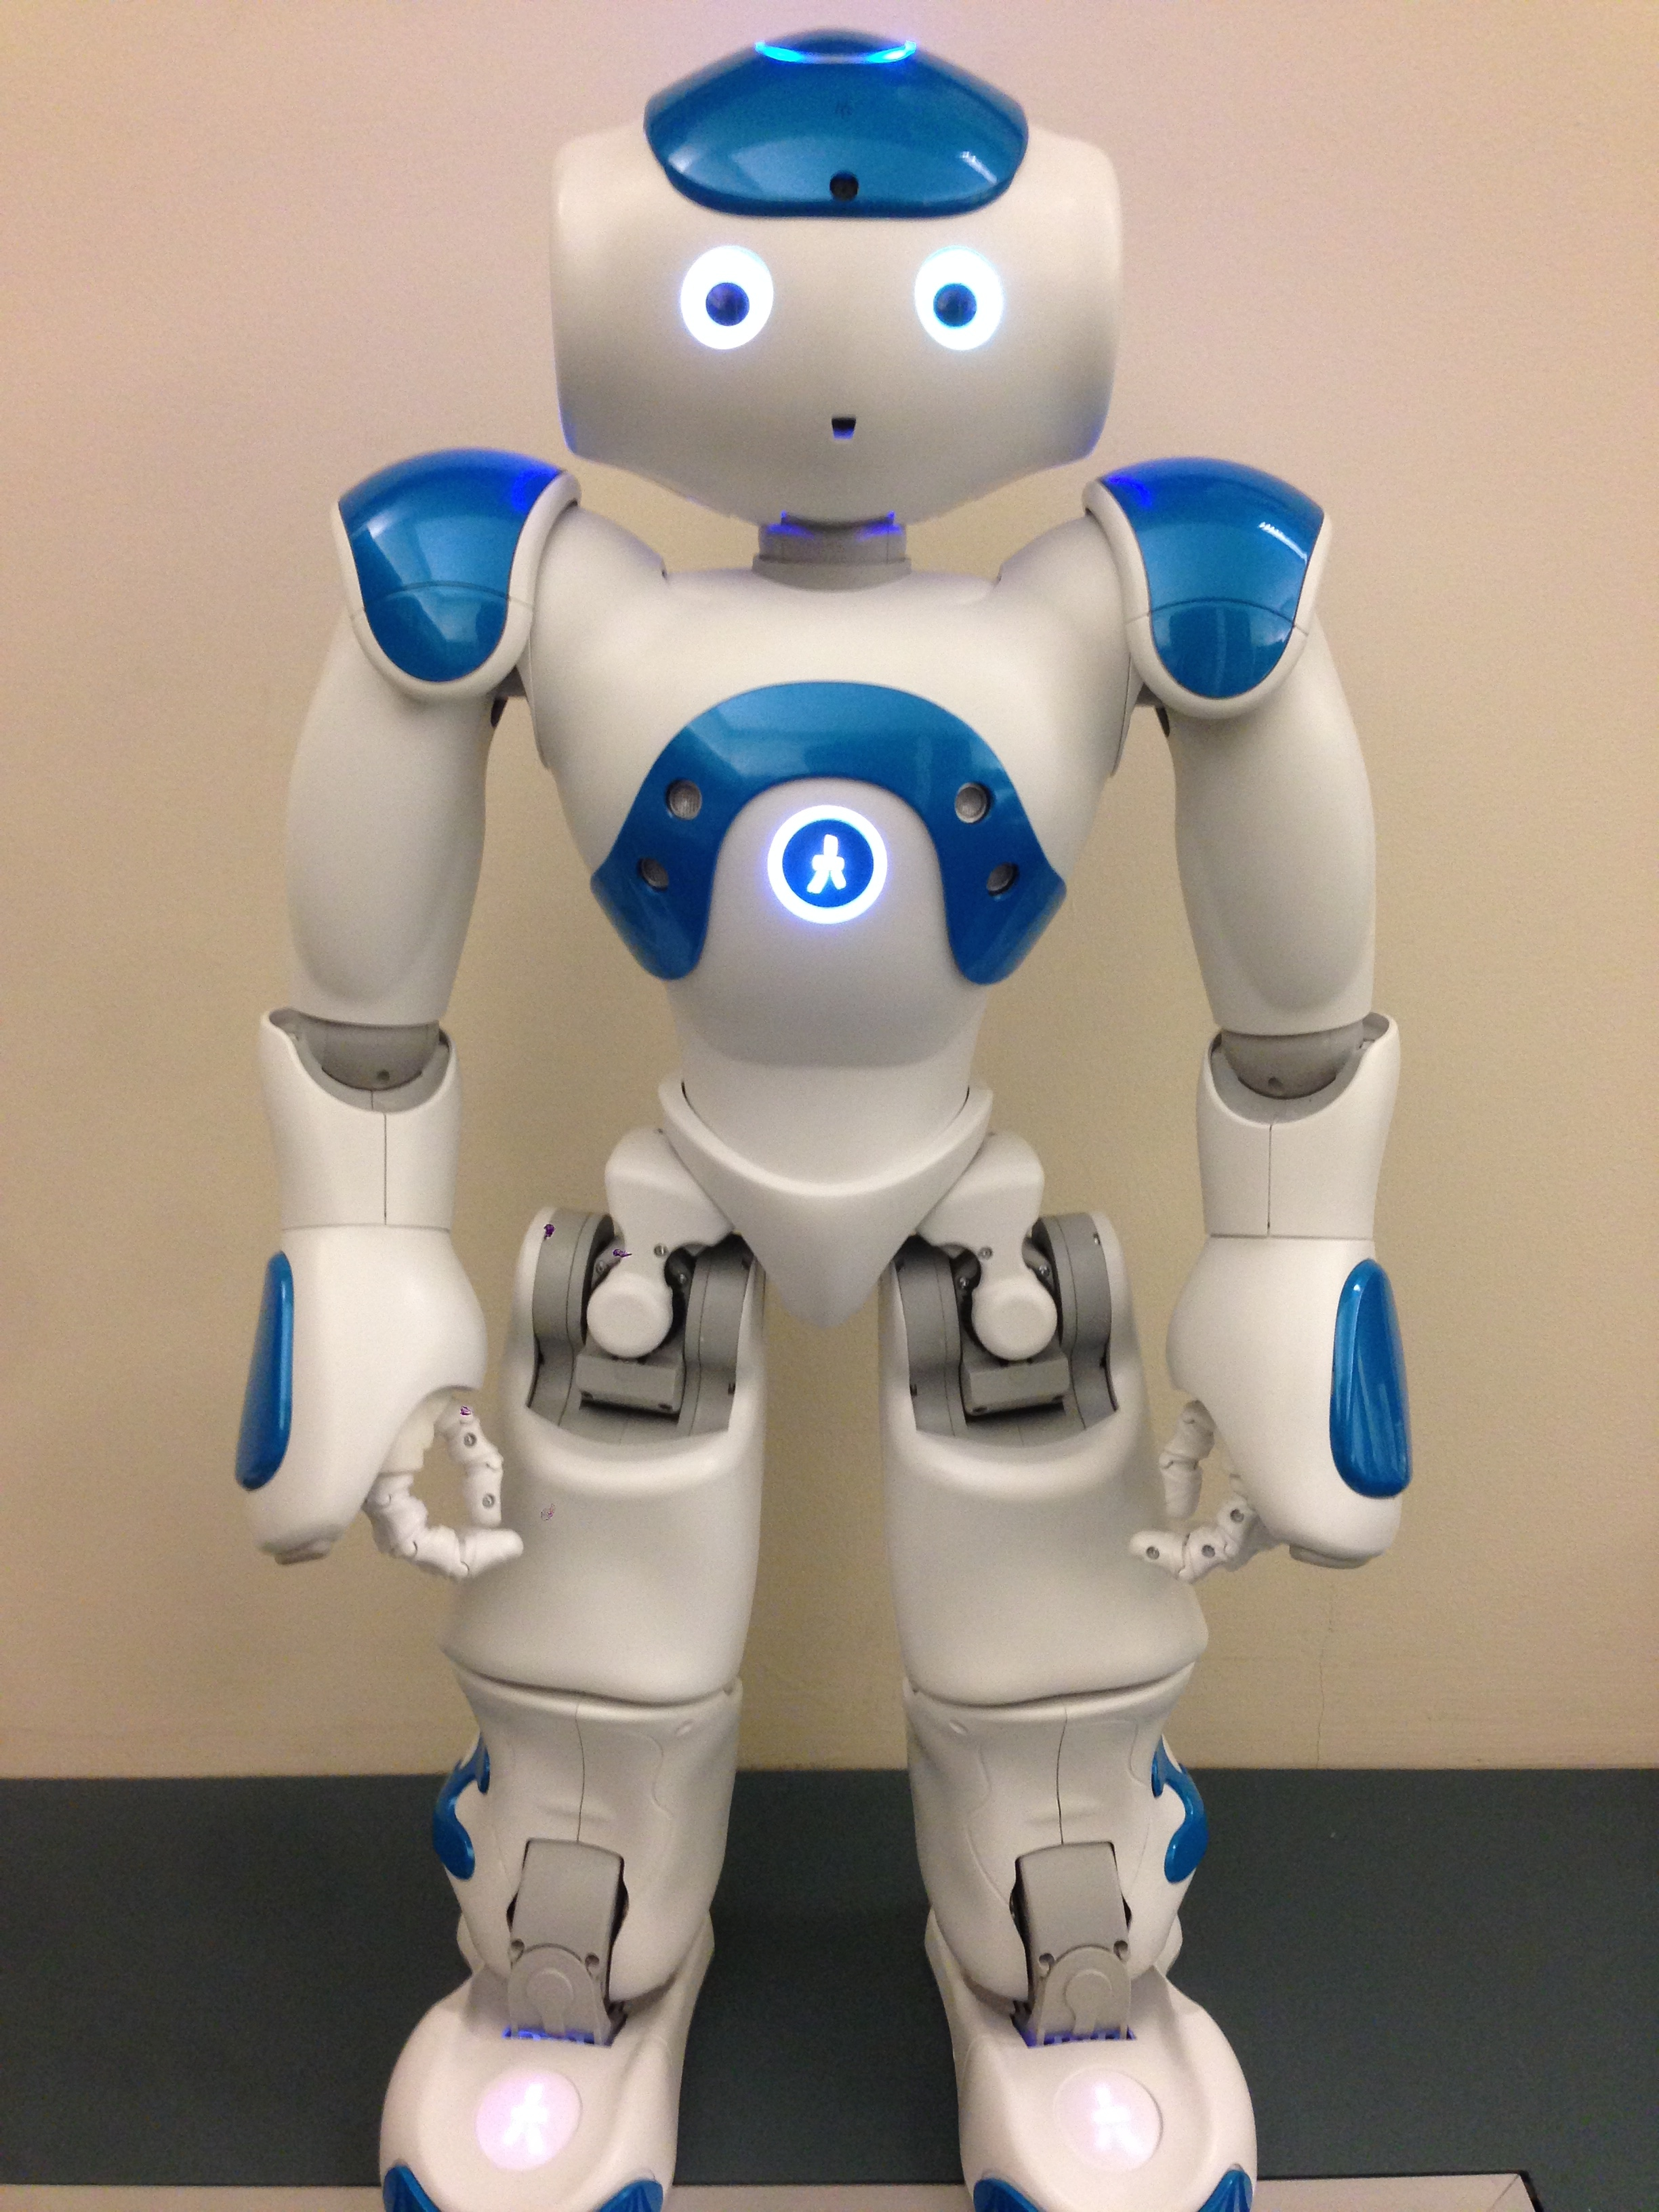
\includegraphics[width=0.65\linewidth]{images/normal3.jpg}\\
% \caption{Standard Nao, No Behavior, ``Before''}
% \label{normal}%\vspace*{-2mm}
%\end{figure}
%
%\begin{figure}[t!]
%\centering
% 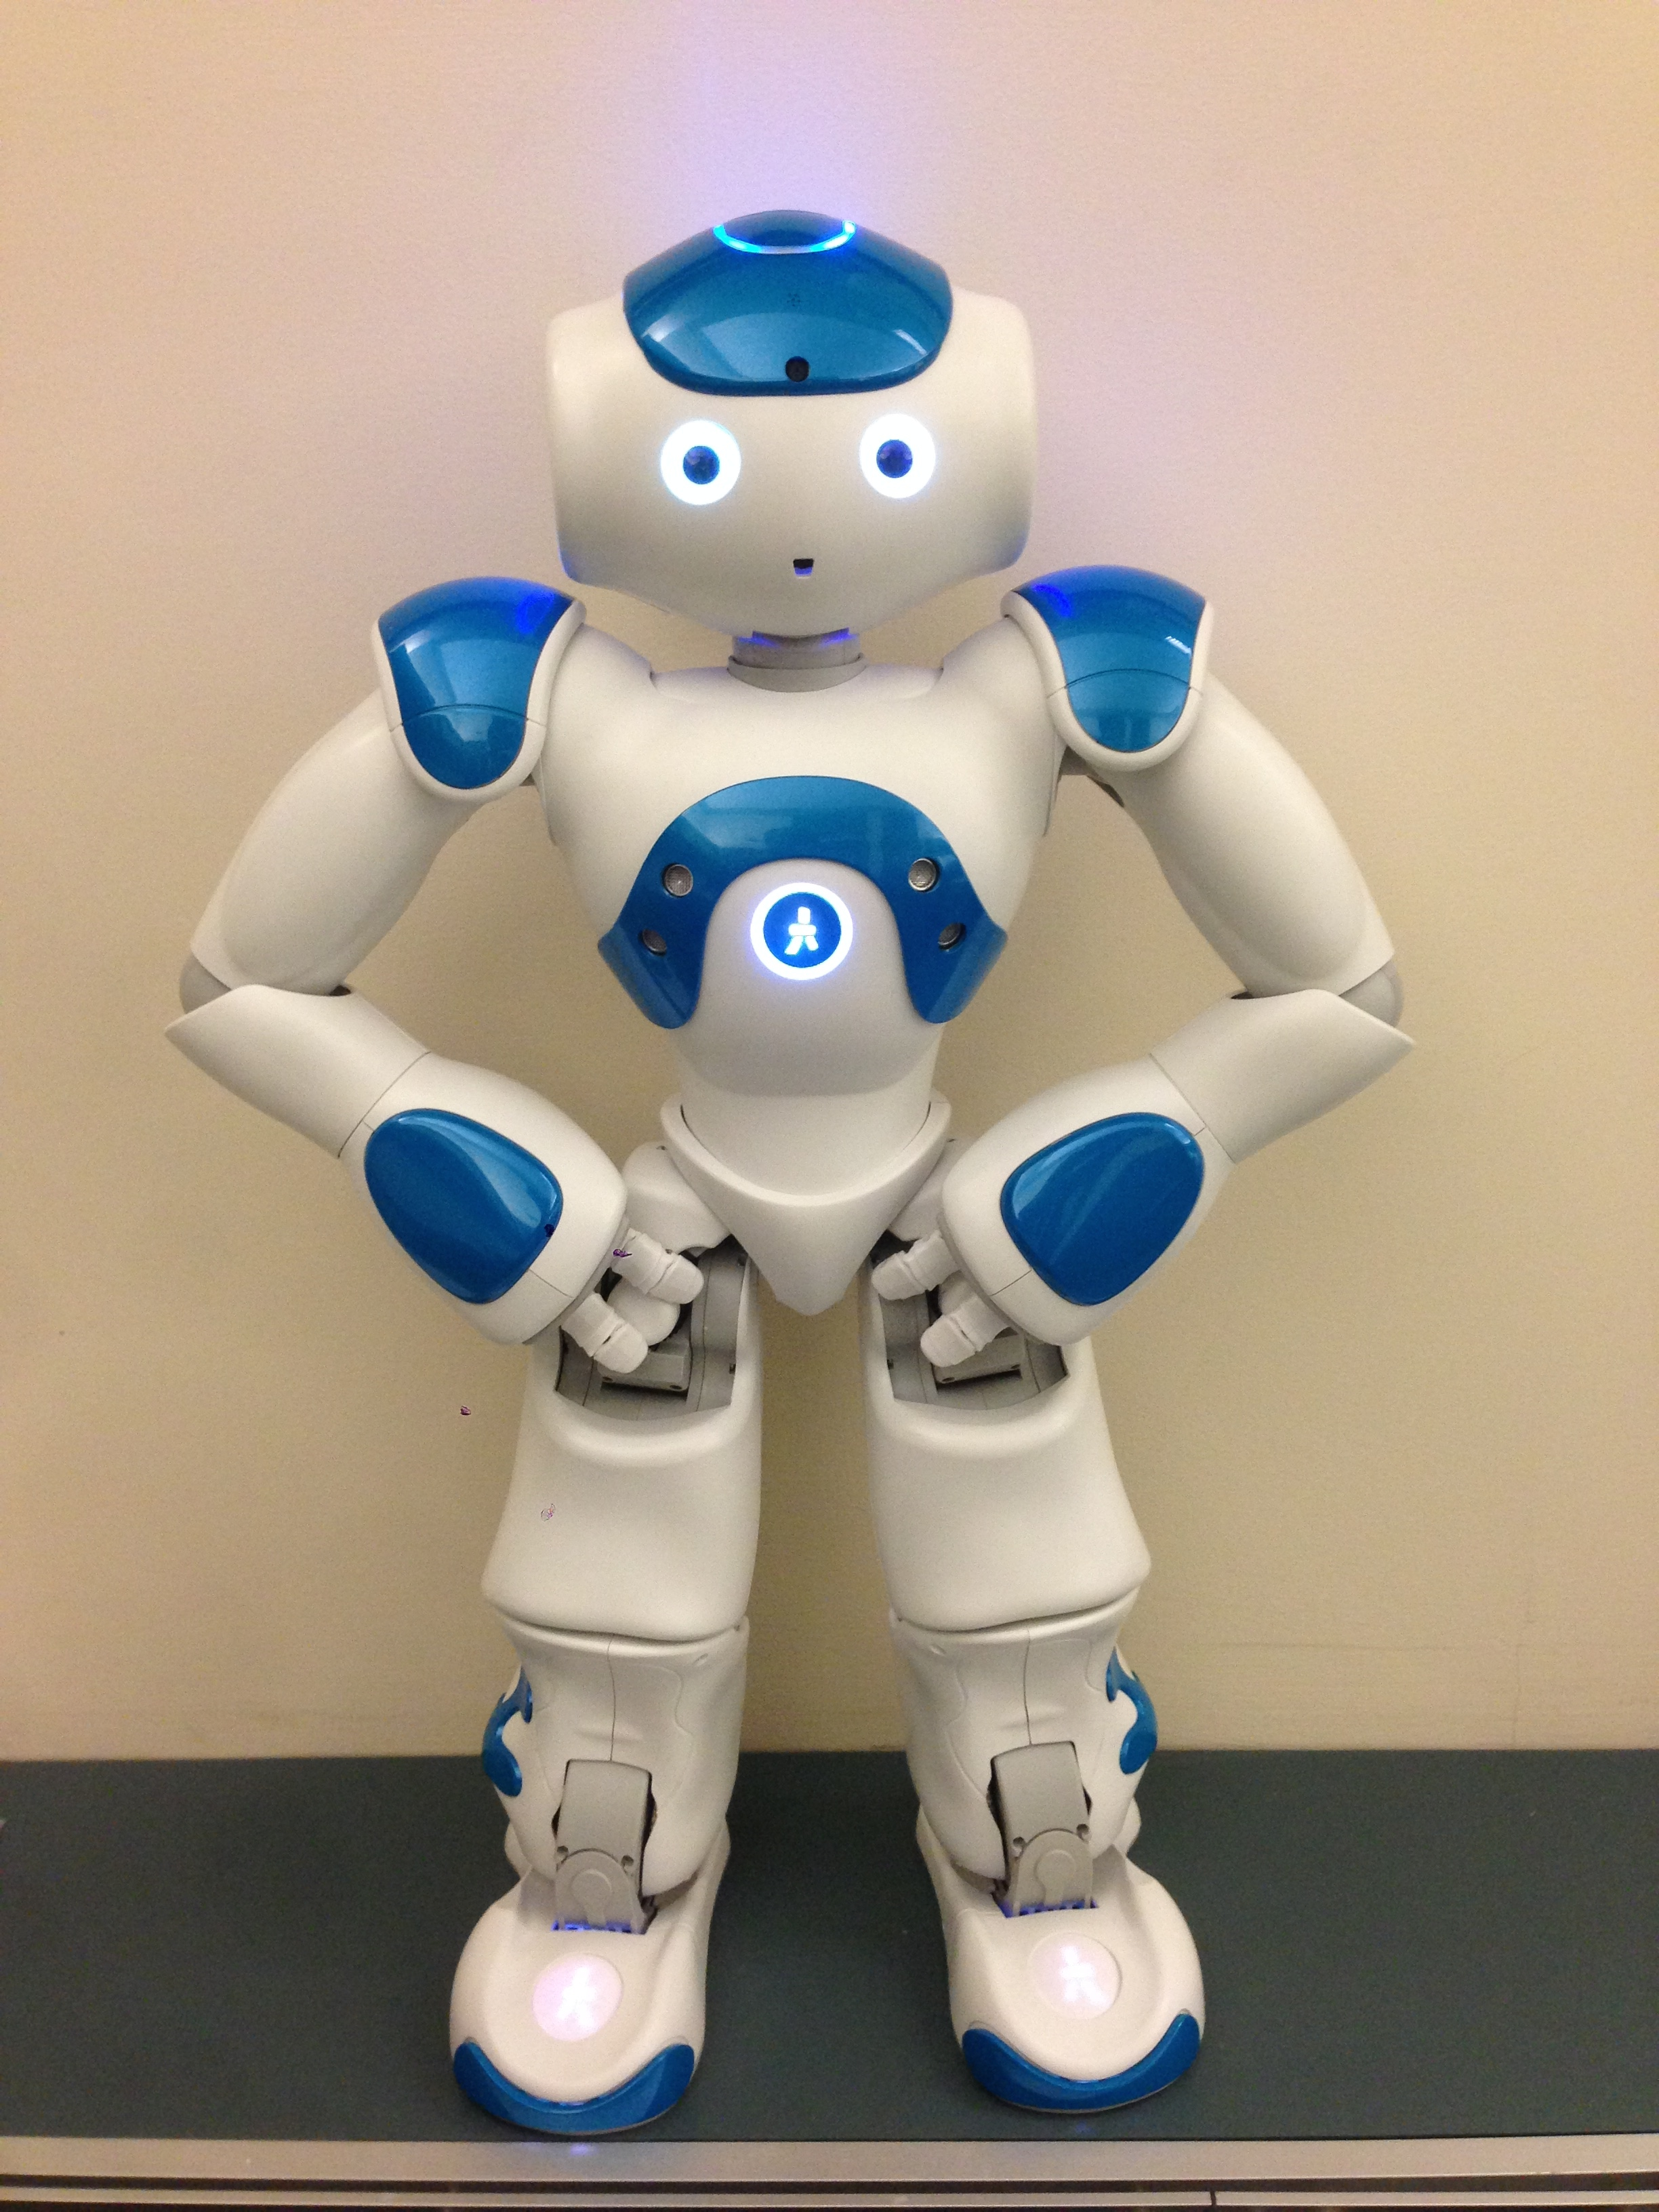
\includegraphics[width=0.65\linewidth]{images/hips7.jpg}\\
% \caption{Nao Robot With Hands on Hips}
% \label{hips} %\vspace*{-2mm}
%\end{figure}
%
%\begin{figure}[t!]
%\centering
% 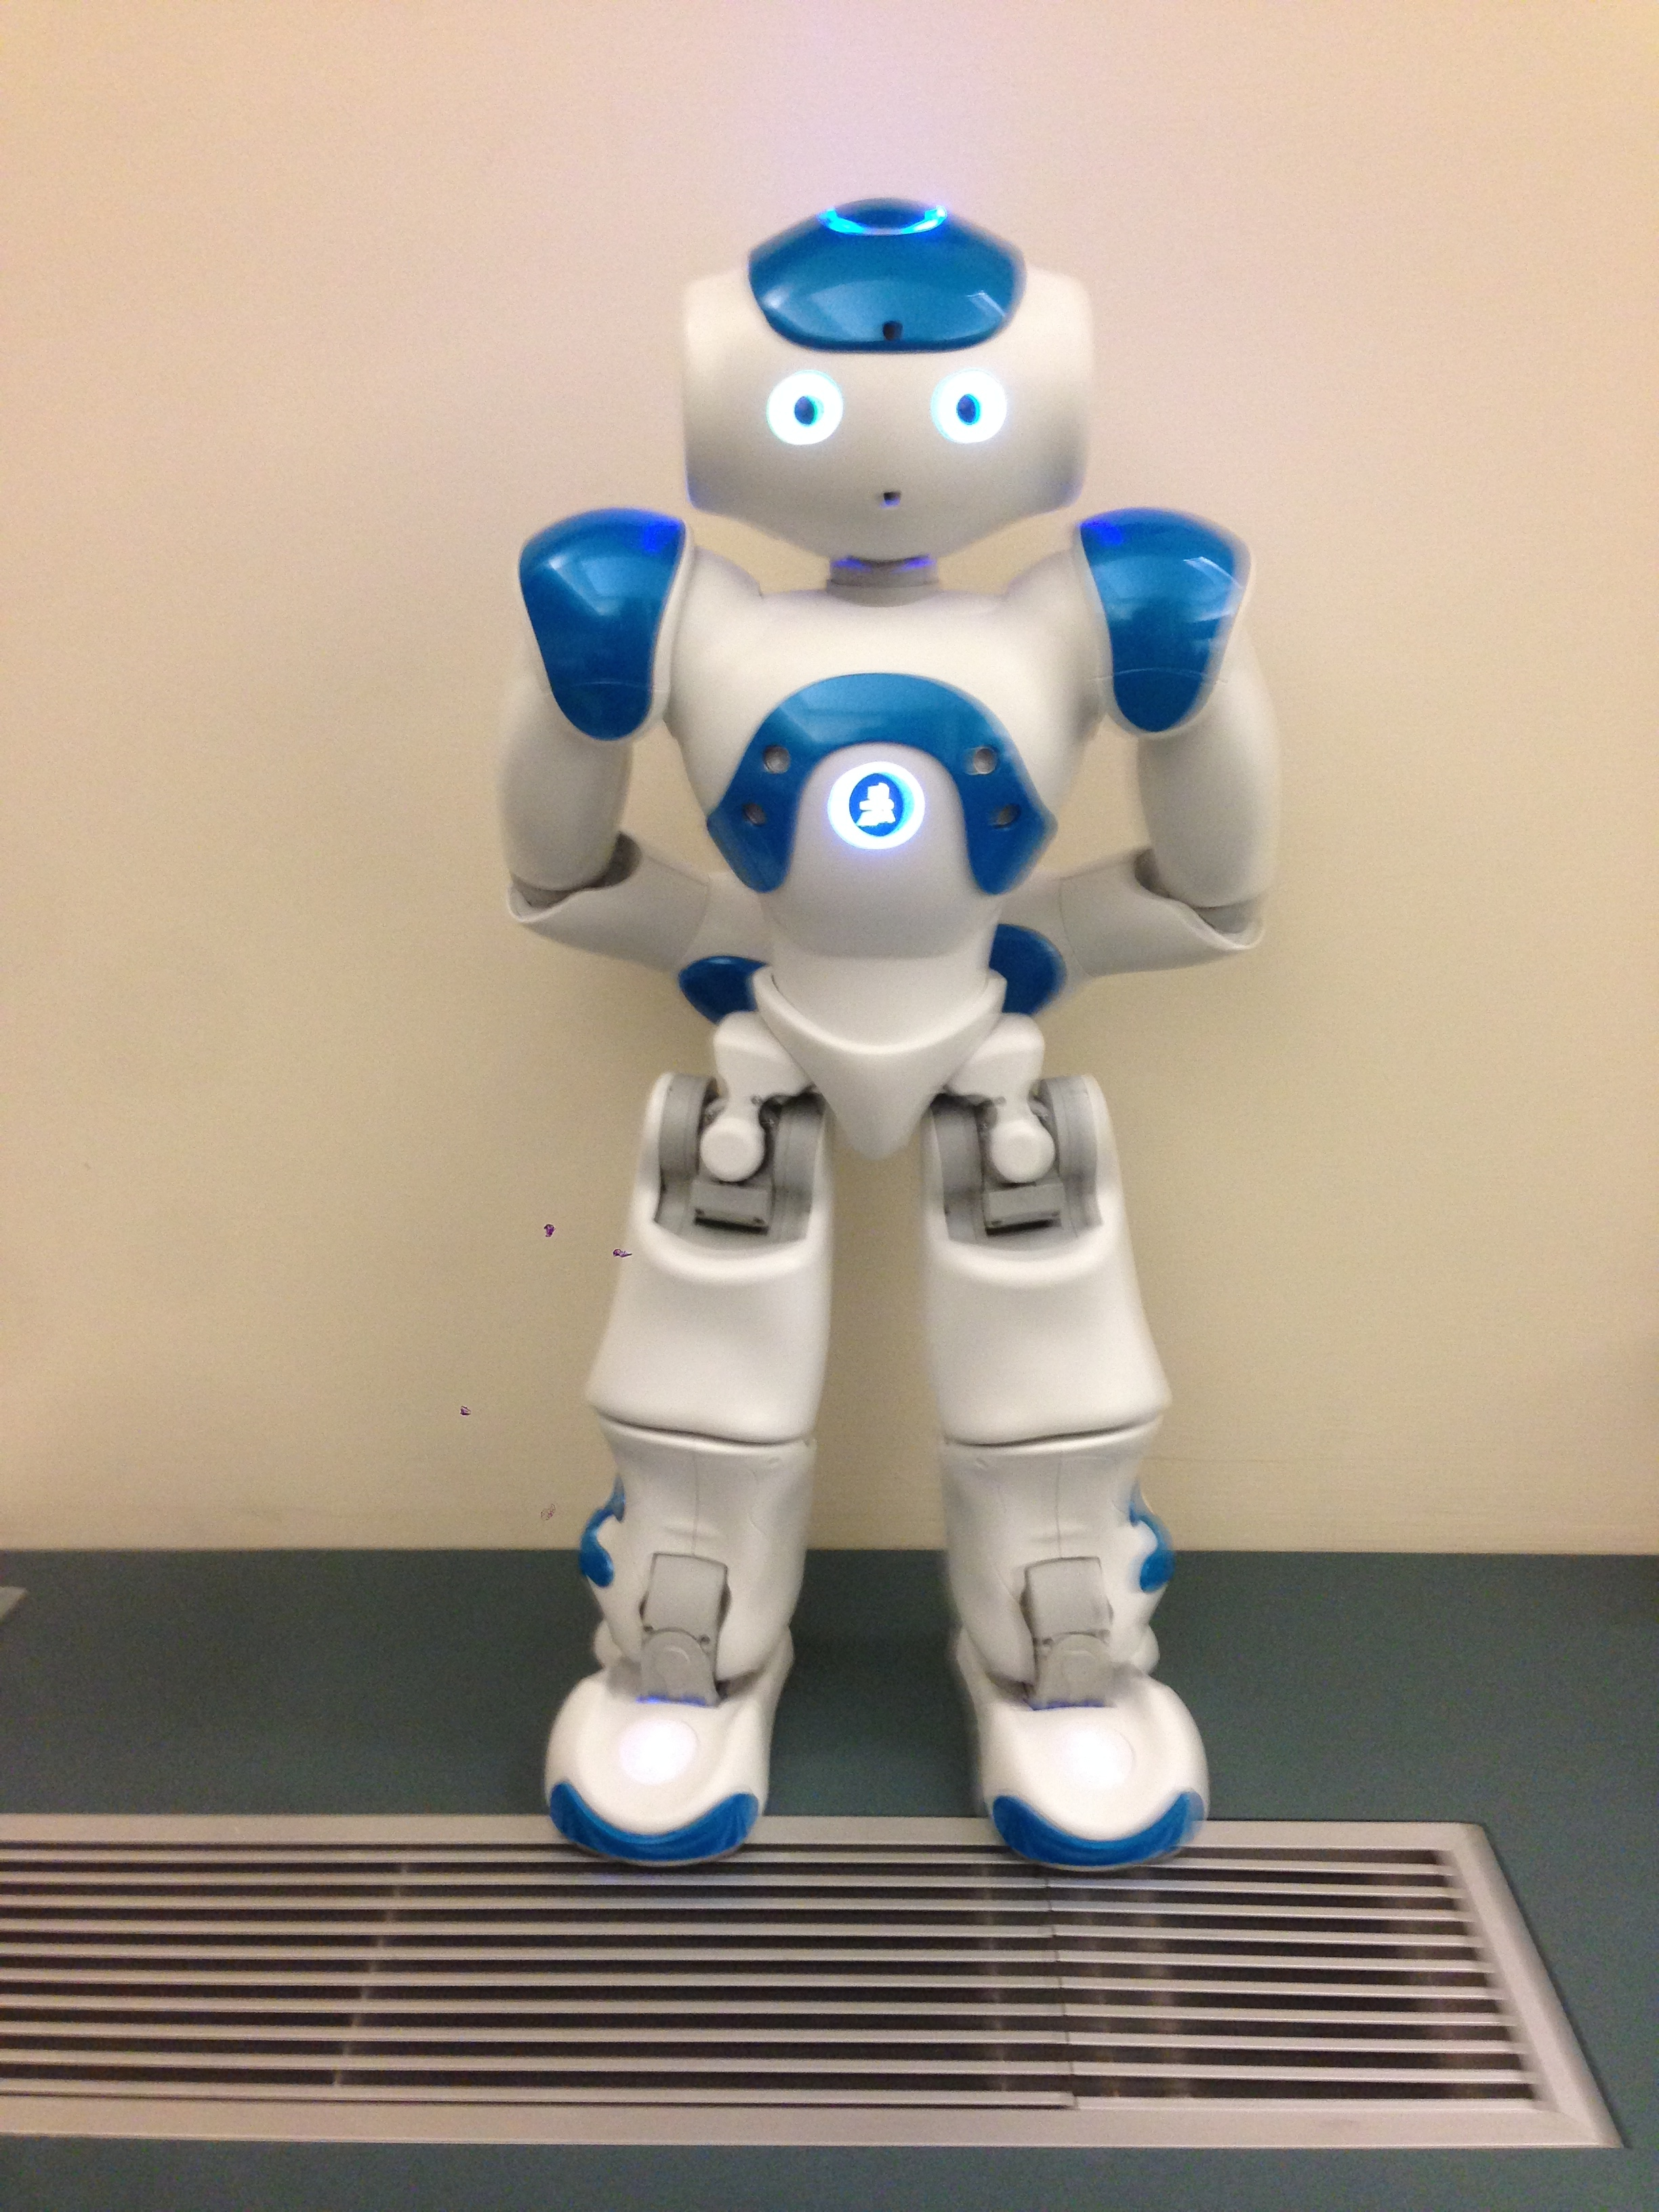
\includegraphics[width=0.65\linewidth]{images/behind3.jpg}\\
% \caption{Nao Robot With Hands Behind Back}
% \label{behind} %\vspace*{-2mm}
%\end{figure}

%\textbf{Video Coding} We coded a participant putting hands on hips with 4 different designations and a participant putting hands behind back with 3 different designations. The different designations ensured we were able to cover all variations of the behaviors in the event they were displayed. For hands on hips the designations were two hands on hips, one hand on hip, hands in pockets, and hands in belt loops. We ultimately did not use hands in pockets or hands in belt loops because they did not accurately resemble the Nao's behavior. For hands behind back the designations were two hands behind back, one hand behind back, and hands in back pockets. We ultimately did not use hands in back pockets because it did not accurately resemble the Nao's behavior.
	
%\textbf{Strict vs. Loose} For our analysis we broke both behaviors into a strict and loose definition. For hands on hips, the strict definition matches the Nao's behavior of putting two hands on hips. The loose definition is a superset of this, with the participant exhibiting \textit{at least} one hand on hip. For hands behind back, the strict definition matches the Nao's behavior of putting two hands behind back. The loose definition is a superset of this, with the participant exhibiting \textit{at least} one hand behind back. Having a strict and loose interpretation allowed us to take into account participants who partially performed the behavior in our analysis. 
%At the start of this study, we hypothesized the following:\\
%\textbf{H1}	People who do not spontaneously exhibit a behavior will perform that behavior more after seeing a robot perform it.\\
%\textbf{H2} People who do spontaneously exhibit a behavior will perform that behavior less after seeing a robot perform it.